\chapter{Experimentación y análisis de resultados} \label{chapter:chapter4}

\section{Baselines supervisados}

Previo a la experimentación con los modelos de redes convolucionales en escalera, era necesario buscar
un punto de comparación de estos modelos con algún baseline. Por lo cuál, se seleccionaron tres baselines
basándonos en una estructura de red neuronal puramente supervisada, es decir, sin utilizar datos no anotados como es el caso de la red en escalera. Estos se detallaron en el Capítulo anterior, y 
a continuación se denotarán los experimentos y mostrarán los resultados de los mismos.

\subsection{Perceptrón multicapa}\label{baseline:mlp}

El primer conjunto de experimentos fue realizado sobre el perceptrón multicapa común, que se describe con 
mayor detalle en la Sección \ref{sec:perceptron}. El conjunto de datos para entrenamiento y evaluación de este
modelo se establecieron en 100000 instancias de entrenamiento y 20000 para evaluación y validación. Para 
conseguir esta muestra de ejemplos primero se realizó una división de los documentos del corpus como se 
detalla en el Cuadro \ref{tab:division}. 

Luego, sobre cada subconjunto de documentos se tomo una muestra aleatoria de las instancias mencionadas 
anteriormente. 

Notar que para estas muestras se realizó un \textit{subsampling} de la clase O tanto para las instancias de
tipo \textit{palabra-etiqueta} como para \textit{fragmento oración-etiqueta}. Esta decisión fue tomada con el
objetivo de balancear las clases.

Para el caso del perceptrón multicapa se muestran tres experimentos, uno para cada estrategia de 
representación, con los hiperparámetros que mejores resultados obtuvieron seleccionados de manera aleatoria.
Estos pueden verse detallados en el Cuadro \ref{tab:exp:perceptron}.

\begin{table}[h]
    \centering
    \begin{tabular}{|l|l|l|}
        \hline
        \textbf{Experimento} & \textbf{Hiperparámetro} & \textbf{Valor} \\
        \hline
        \multirow{4}{*}{MLP.1} & Representación & Promedio \\
                               & Ventana & 5 \\
                               & Capas & [300, 256, 128, 5] \\
                               & Tasa de aprendizaje & 0.3 \\
        \hline
        \multirow{4}{*}{MLP.2} & Representación & Decaimiento fraccional \\
                               & Ventana & 5 \\
                               & Capas & [300, 256, 128, 5] \\
                               & Tasa de aprendizaje & 0.3 \\
        \hline
        \multirow{4}{*}{MLP.3} & Representación & Decaimiento exponencial \\
                               & Ventana & 5 \\
                               & Capas & [300, 256, 128, 5] \\
                               & Tasa de aprendizaje & 0.3 \\
        \hline
    \end{tabular}
    \caption{Hiperparámetros del conjunto de experimentos con perceptrón multicapa supervisado.}
    \label{tab:exp:perceptron}
\end{table}

\subsubsection{Resultados}

La Figura \ref{fig:MLPbaselines} muestra los resultados de aplicar los tres experimentos detallados en el
Cuadro \ref{tab:exp:perceptron}. Es un gráfico de barras con agrupación. El eje $y$ del gráfico muestra la
exactitud ({\em accuracy}) del experimento, donde a mayor valor, mejor el resultado. 

Por otro lado, el eje $x$ representa la estrategia aplicada (i.e. el experimento de acuerdo al Cuadro 
\ref{tab:exp:perceptron}), agrupando tres barras de acuerdo al conjunto de datos sobre el que se muestra el 
resultado. De esta manera, la barra azul muestra el resultado sobre el conjunto de entrenamiento, la barra 
naranja sobre el conjunto de validación y la barra verde sobre el conjunto de evaluación ({\em test}).

\begin{figure}[t]
\begin{center}
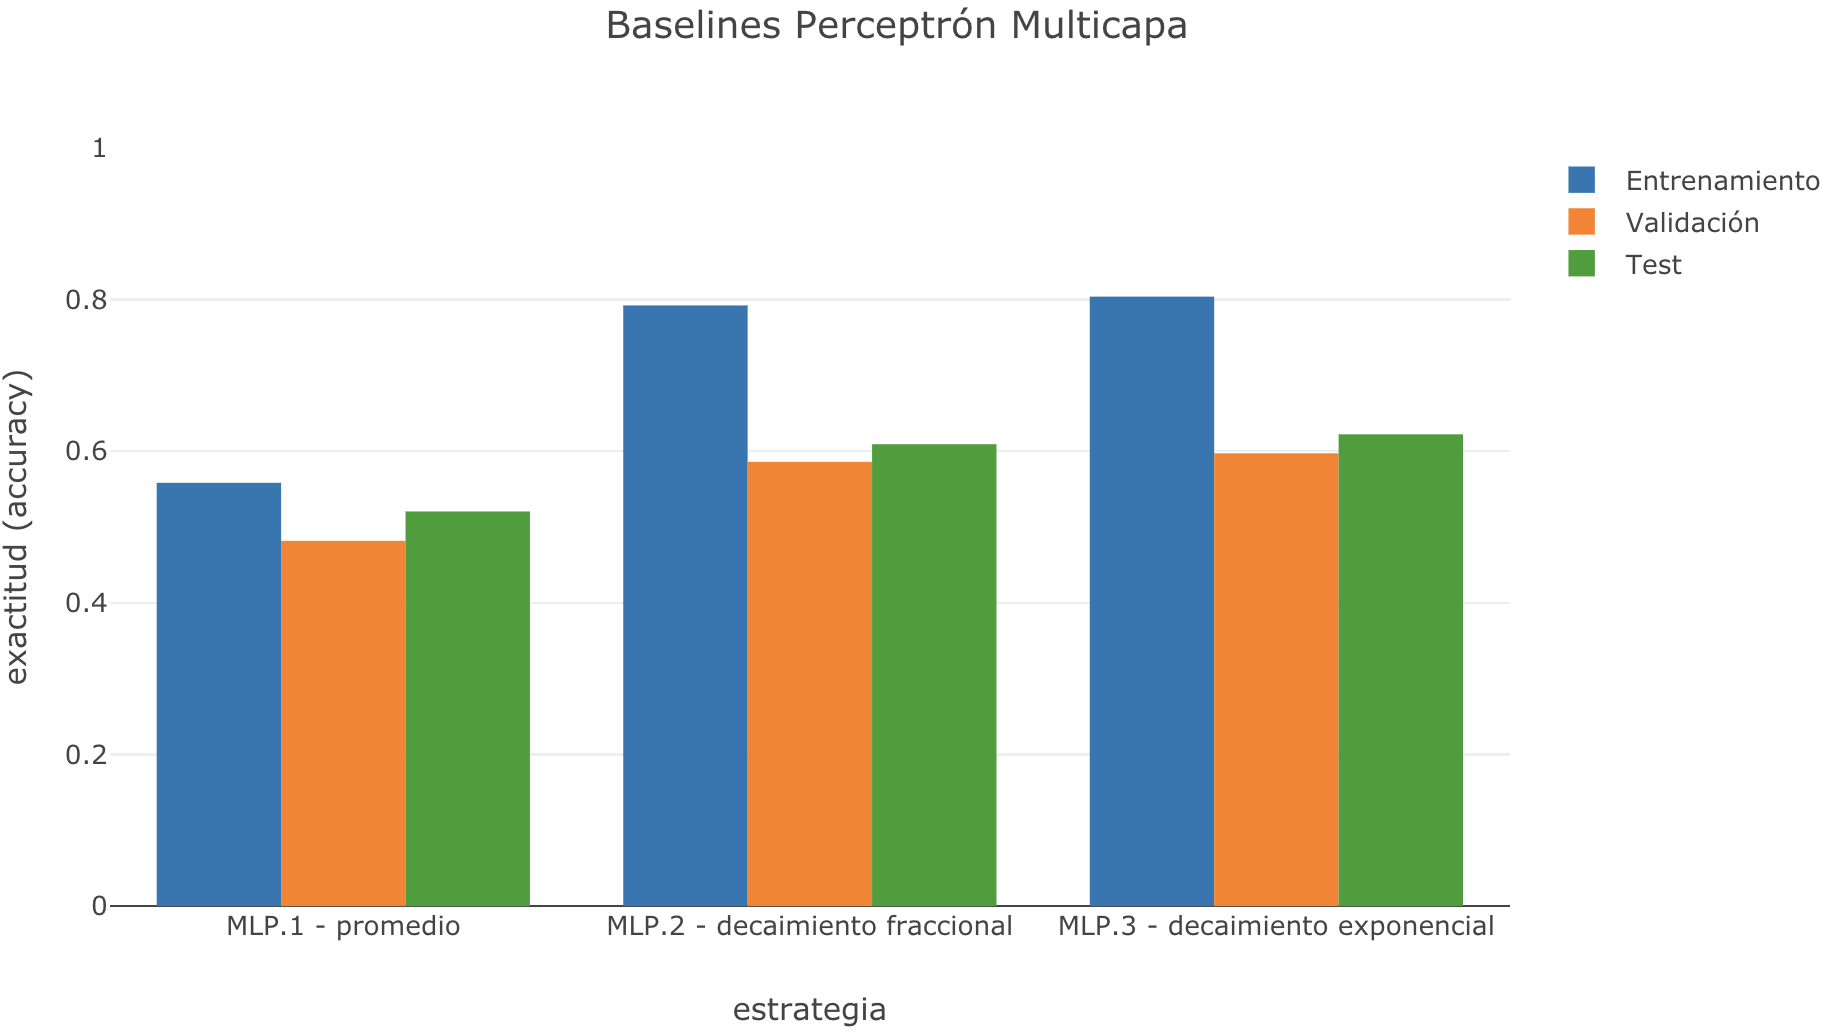
\includegraphics[width=.9\linewidth]{images/MLP_baselines.png}
\caption{Resultados de los experimentos MLP. Comparación utilizando distintas representaciones de datos de 
entrada.}
\label{fig:MLPbaselines}
\end{center}
\end{figure}

Como se puede observar en la Figura \ref{fig:MLPbaselines}, utilizar el decaimiento exponencial y fraccional 
como estrategias de representación de una palabra son una buena alternativa. 

Esto posiblemente se deba a que la información de contexto que le aporta una palabra inmediatamente vecina a 
la palabra objetivo es mucho más relevante que una más distante. 

Por otro lado, simplemente tomar el promedio de las palabras circundantes no tiene buenos resultados y 
justamente no tiene en cuenta lo mencionado anteriormente. De estos experimentos el experimento MLP.3 es el 
que mejor resultados obtiene y es el seleccionado para su comparación en los experimentos mostrados en las 
siguientes secciones.

\subsection{Redes convolucionales en amplitud}\label{baseline:cnn:wide}

Para estos experimentos un ejemplo de entrenamiento es un fragmento de oración como se detalla en la Sección 
\ref{sec:fragmento_sentencia}. 

El conjunto de datos para el entrenamiento y evaluación de este modelo se establecieron 100000 instancias de 
entrenamiento y 20000 para validación y evaluación de manera análoga a los experimentos anteriores. 

El Cuadro \ref{tab:exp:cnn_wide_supervised} establece la lista de experimentos e hiperparámetros utilizados. 
El objetivo los experimentos es analizar si el modelo sufre variaciones al utilizar diferentes proporciones de
instancias de entrenamiento anotadas.

\begin{table}[h]
    \centering
    \begin{tabular}{|l|l|l|}
        \hline
        \textbf{Experimento} & \textbf{Hiperparámetro} & \textbf{Valor} \\
        \hline
        \multirow{7}{*}{Hiper. generales} & Ventana simétrica W & 2 \\
                              & Número de filtros & 100 \\
                              & Tamaño de max pooling & 1 \\
                              & Tamaño de kernels & [2,3,4] \\
                              & Dropout & 0.5 \\
                              & Capas densas & [128, 5] \\
                              & Regularizador L2 & 1 \\
        \hline
        \multirow{1}{*}{CNN-Wide-Sup.1} & \% ejemplos entrenamiento & 25\% \\
        \hline
        \multirow{1}{*}{CNN-Wide-Sup.2} & \% ejemplos entrenamiento & 50\% \\
        \hline
        \multirow{1}{*}{CNN-Wide-Sup.3} & \% ejemplos entrenamiento & 75\% \\
        \hline
        \multirow{1}{*}{CNN-Wide-Sup.4} & \% ejemplos entrenamiento & 100\% \\
        \hline
    \end{tabular}
    \caption{Hiperparámetros para CNN Supervisado en Amplitud.}
    \label{tab:exp:cnn_wide_supervised}
\end{table}

\subsubsection{Resultados}

La Figura \ref{fig:CNN_wide_baselines_ratios} muestra los resultados de aplicar los cuatro experimentos 
detallados en el Cuadro \ref{tab:exp:cnn_wide_supervised}. Se observan las curvas correspondientes al valor de
exactitud que logra cada modelo a lo largo de las épocas de entrenamiento. Se utiliza el color azul para 
denotar la exactitud en los datos de entrenamiento mientras que el anaranjado para los datos de validación. No
se observan diferencias significativas al utilizar una menor cantidad de datos anotados para el entrenamiento 
del modelo. Más adelante se tendrá en consideración el experimento CNN-Wide-Sup.4 que utiliza el 100\% de las 
instancias de entrenamiento para su comparación con el equivalente en la versión en escalera.

\begin{figure}[t]
\begin{center}
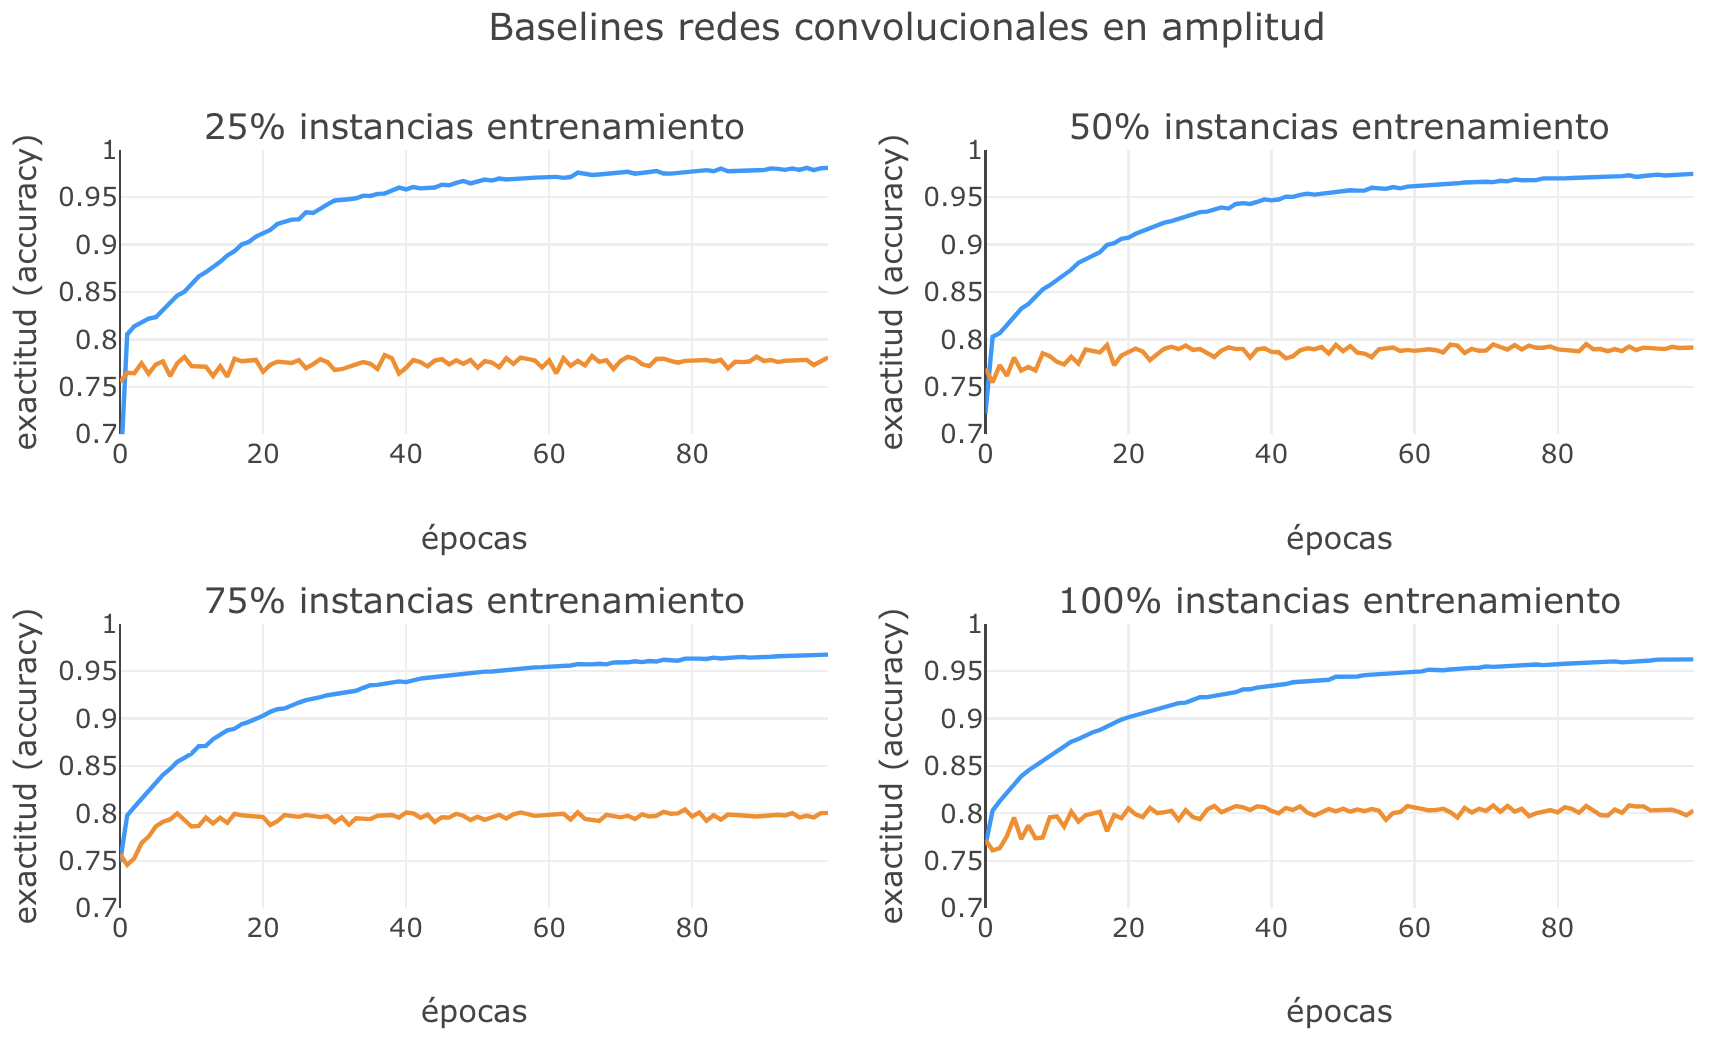
\includegraphics[width=.9\linewidth]{images/CNN_wide_baselines_ratios.png}
\caption{Resultados redes convolucionales en amplitud. Comparación utilizando distintas porciones de corpus
como datos de entrenamiento para el modelo.}
\label{fig:CNN_wide_baselines_ratios}
\end{center}
\end{figure}

\subsection{Redes convolucionales en profundidad}\label{baseline:cnn:deep}

Para estos experimentos la entrada del modelo es una oración y la salida una secuencia de etiquetas que se 
corresponde una a una con cada \textit{token} de la oración ingresada tal como se detalla en la Sección 
\ref{sec:sequence_labeling}. 

El conjunto de datos para el entrenamiento y evaluación de este modelo se establecieron 100000 instancias de 
entrenamiento y 20000 para validación y evaluación. Para este caso en el que las instancias son oraciones y no
palabras no se realiza un \textit{subsampling} de la clase mayoritaria O, por lo que el conjunto de datos se 
presenta inherentemente desbalanceado. 

Para el caso del modelo de redes convolucionales en profundidad supervisado se muestran cuatro experimentos, 
con los hiperparámetros que mejores resultados obtuvieron seleccionados de manera aleatoria. En particular, se
busca ver si el uso de varias capas convolucionales mejora el desempeño del modelo. Estos pueden verse 
detallados en el Cuadro \ref{tab:exp:cnn_depth_supervised}.

\begin{table}[h]
    \centering
    \begin{tabular}{|l|l|l|}
        \hline
        \textbf{Experimento} & \textbf{Hiperparámetro} & \textbf{Valor} \\
        \hline
        \multirow{3}{*}{Hiper. generales} & Tamaño de kernels & 2 \\
                              & Dropout & 0 \\
                              & Regularizador L2 & 0 \\
        \hline
        \multirow{2}{*}{CNN-Depth-Sup.1} & Capas convolucionales & 3 \\
                                         & Número de filtros por capa & 50 \\
        \hline
        \multirow{2}{*}{CNN-Depth-Sup.2} & Capas convolucionales & 10 \\
                                         & Número de filtros por capa & 50 \\
        \hline
        \multirow{2}{*}{CNN-Depth-Sup.3} & Capas convolucionales & 3 \\
                                         & Número de filtros por capa & 100 \\
        \hline
        \multirow{2}{*}{CNN-Depth-Sup.4} & Capas convolucionales & 5 \\
                                         & Número de filtros por capa & 100 \\
        \hline
    \end{tabular}
    \caption{Hiperparámetros del conjunto de experimentos con redes convolucionales en profundidad 
    supervisado.}
    \label{tab:exp:cnn_depth_supervised}
\end{table}

\subsubsection{Resultados}

\begin{figure}[t]
\begin{center}
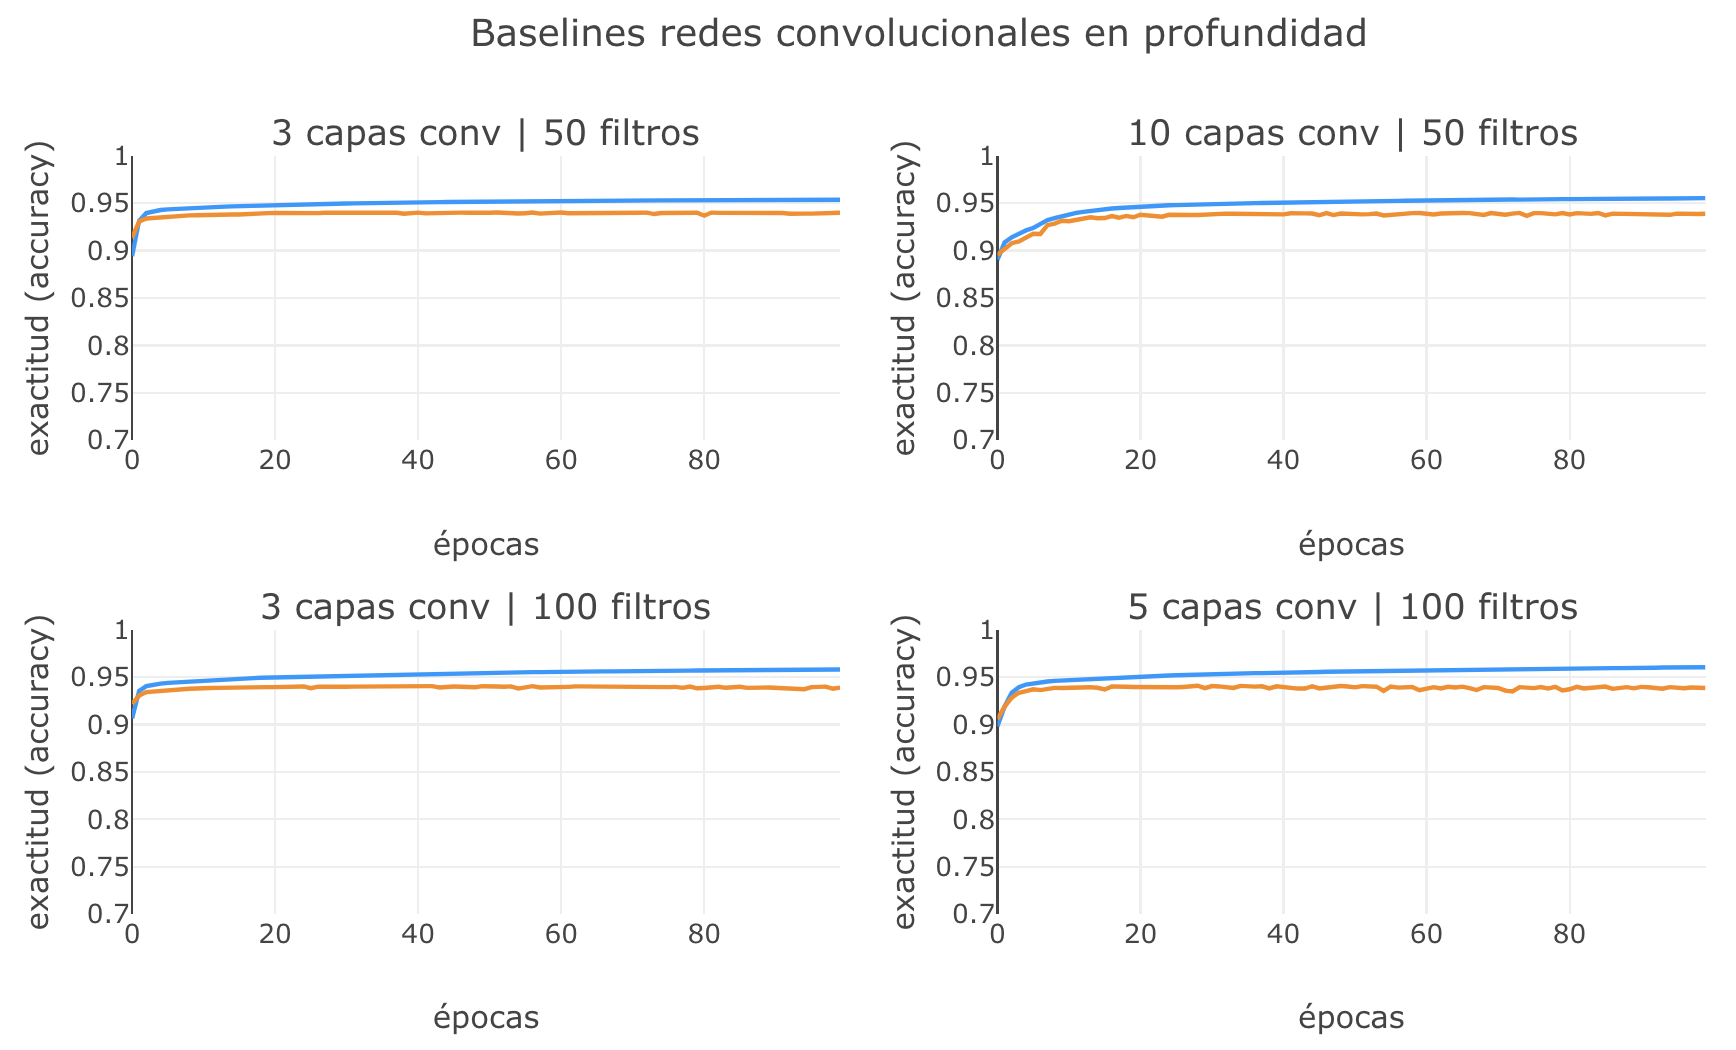
\includegraphics[width=.9\linewidth]{images/CNN_depth_baselines.png}
\caption{Resultado redes convolucionales en profundidad supervisado. Comparación utilizando
distinta cantidad de capas convolucionales y cantidad de filtros por capa.}
\label{fig:CNN_depth_baselines}
\end{center}
\end{figure}

En la Figura \ref{fig:CNN_depth_baselines} se observan cuatro experimentos, los cuales representan los mejores
resultados de los distintos experimentos que se ejecutaron sobre este modelo supervisado. 

Nuevamente el color azul denota el valor de exactitud en los datos de entrenamiento y el anaranjado para el 
caso de los datos de validación. Un aspecto a tener en cuenta es que utilizar como métrica la exactitud para 
su comparación con los modelos anteriores es algo que hay que trabajar con cuidado, ya que al manejar 
instancias a nivel de oración las clases se encuentran inherentemente desbalanceadas, por lo que la exactitud 
puede ser alta simplemente marcando todo como la clase mayoritaria.

Sin embargo, por cuestiones comparativas, sobre todo con los modelos anteriores, se utiliza el experimento 
CNN-Depth-Sup.2 para dicha tarea y con su variante implementación en escalera (en la Figura 
\ref{fig:CNN_depth_baselines}, el de arriba a la derecha, con 10 capas convolucionales y 50 filtros por capa).

\subsection{Comparación de baselines}

Al obtener los mejores hiperparámetros para los modelos baseline, se decidió compararlos para tener una idea 
clara de lo que estamos tratando de lograr superar con la ayuda de las redes en escalera. Para esto, el método
de comparación es con el conjunto de datos de evaluación, en lugar del conjunto de datos de validación.

La Figura \ref{fig:best_supervised_baselines} compara los resultados de los mejores modelos de cada variante 
supervisada. Es un gráfico de barras con agrupación. El eje $y$ del gráfico muestra la exactitud ({\em 
accuracy}) del experimento, donde a mayor valor, mejor el resultado. Por otro lado,
el eje $x$ representa cada uno de los mejores experimentos, 
agrupando tres barras de acuerdo al conjunto de datos sobre el que se muestra el resultado. De esta manera, la
barra azul muestra el resultado sobre el conjunto de entrenamiento y la barra verde sobre el conjunto de 
evaluación ({\em test}).

En la Figura \ref{fig:best_supervised_baselines} se puede observar la notable mejora que aportan los modelos 
basados en redes convolucionales. Se valida el hecho de que aplicar capas convolucionales provoca que se 
capture información del contexto de cada palabra generando buenos atributos ({\em features}) intermedios que 
el modelo utiliza para la tarea de clasificación de entidades nombradas. 

En otras palabras, el uso de capas convolucionales con la finalidad de extraer características del entorno de 
una palabra parece ser una muy buena alternativa.

Por otro lado, se observa que las redes convolucionales en profundidad arrojan los mejores resultado. De todas
maneras, cabe recordar que el uso de exactitud puede esconder el desempeño del modelo para clases 
minoritarias, por lo que hay que tomarlo con cuidado.

\begin{figure}[t]
\begin{center}
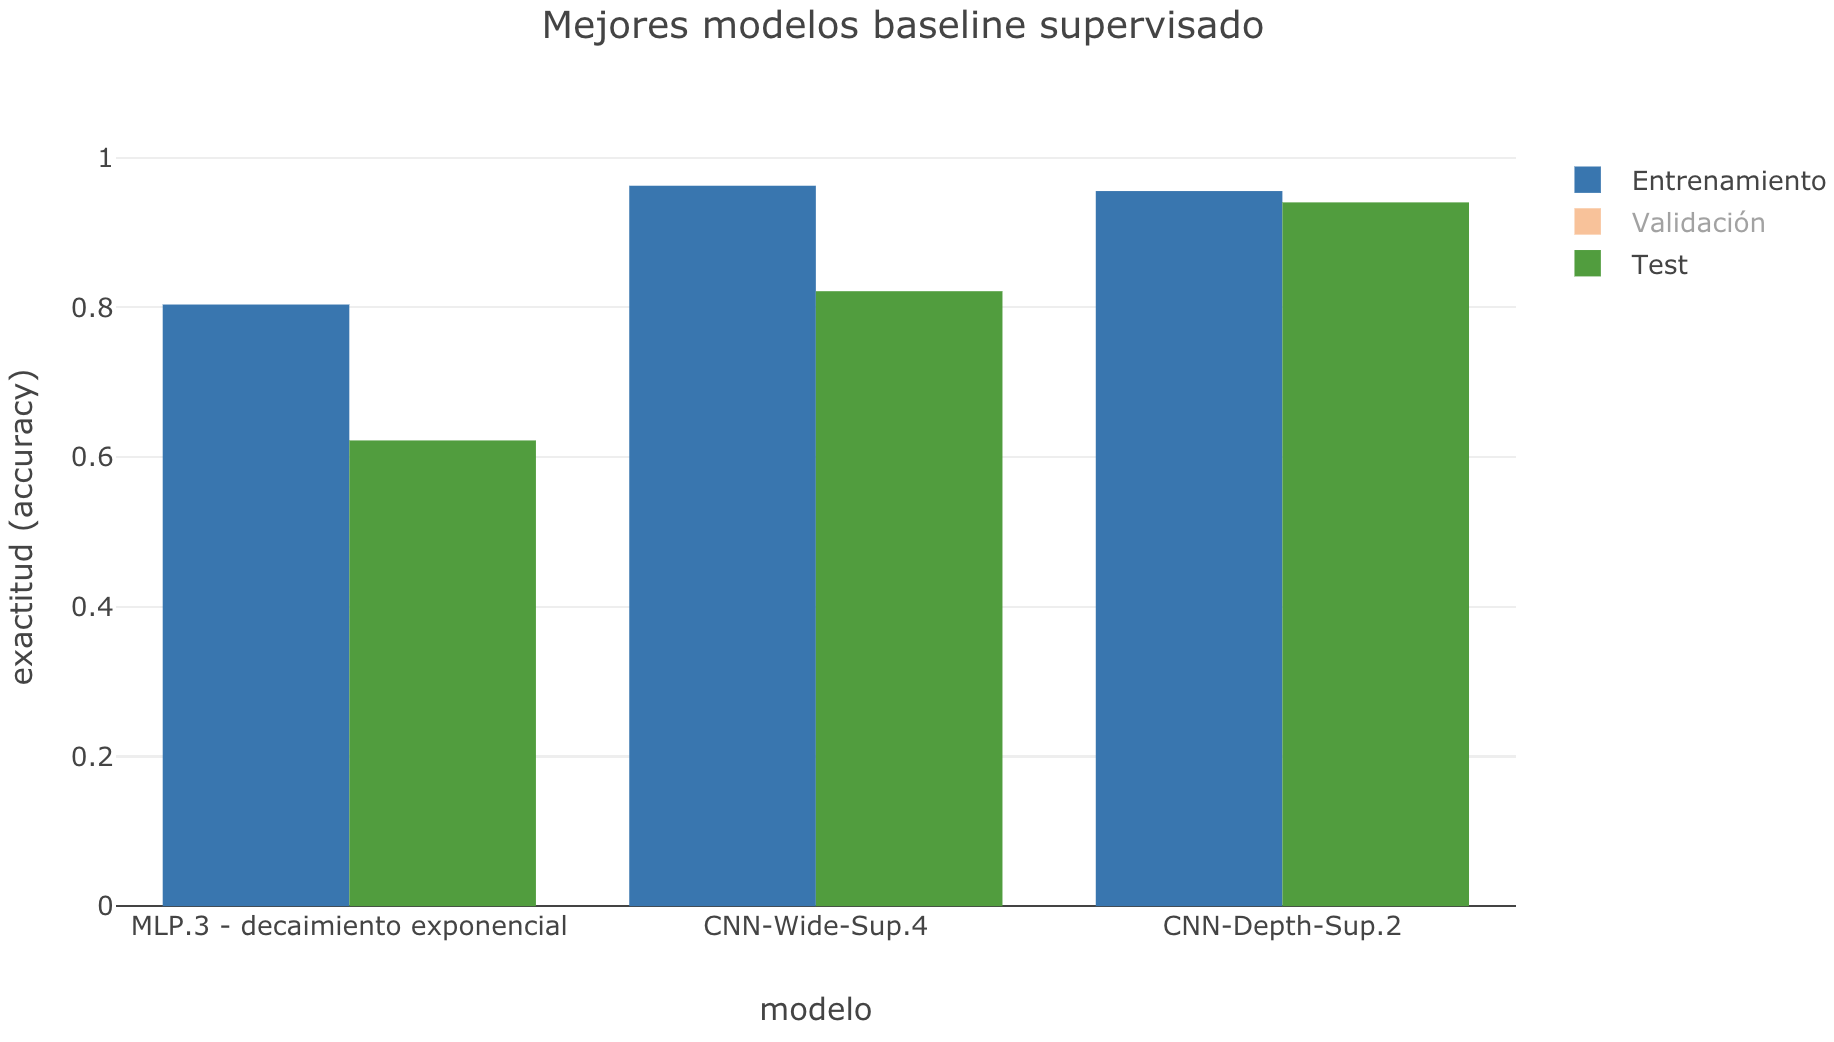
\includegraphics[width=.9\linewidth]{images/best_supervised_baselines.png}
\caption{Mejores modelos baseline supervisados. Comparación de resultados entre datos de entrenamiento y
datos de evaluación}
\label{fig:best_supervised_baselines}
\end{center}
\end{figure}

\section{Redes neuronales en escalera}

Una vez realizados los experimentos netamente supervisados a modo de baseline se prosiguió con la 
incorporación de la tarea no supervisada al utilizar las redes en escalera. Para cada variante se utilizó la 
misma división y conjunto de datos que en los experimentos anteriores, de manera tal que el impacto de los
datos no supervisados pudiese ser medido acorde al experimento realizado.

\subsection{Impacto de los datos no anotados: Perceptrón multicapa en escalera}

En primer lugar, se desea medir el impacto de la tarea no supervisada que brinda la arquitectura en escalera. 
Al incorporar al entrenamiento la utilización de datos no anotados queremos observar si efectivamente derivan 
en una mejora de rendimiento de la red en escalera más básica: el perceptrón multicapa.

Se seleccionó el experimento con mejores resultados del modelo de perceptrón multicapa en escalera para su 
inmediata comparación con su versión supervisada. El Cuadro \ref{tab:exp:mlp_ladder} muestra los 
hiperparámetros de dicho experimento.

\begin{table}[t]
    \centering
    \begin{tabular}{|l|l|l|}
        \hline
        \textbf{Experimento} & \textbf{Hiperparámetro} & \textbf{Valor} \\
        \hline
        \multirow{5}{*}{MLP-Ladder.1} & Representación & Decaimiento exp. \\
                              & Ventana & 5 \\
                              & Capas & [300, 256, 128, 5] \\
                              & Factor de ruido por capa & 0.3 \\
                              & Costo de reducción de ruido & [100, 0.1, 0.1, 0.01] \\
                              & Tasa de aprendizaje & 0.02 \\
        \hline
    \end{tabular}
    \caption{Hiperparámetros del conjunto de experimentos con perceptrón multicapa en escalera.}
    \label{tab:exp:mlp_ladder}
\end{table}

\subsubsection{Evolución de datos de entrenamiento vs. validación a través de épocas}

\begin{figure}[t]
\begin{center}
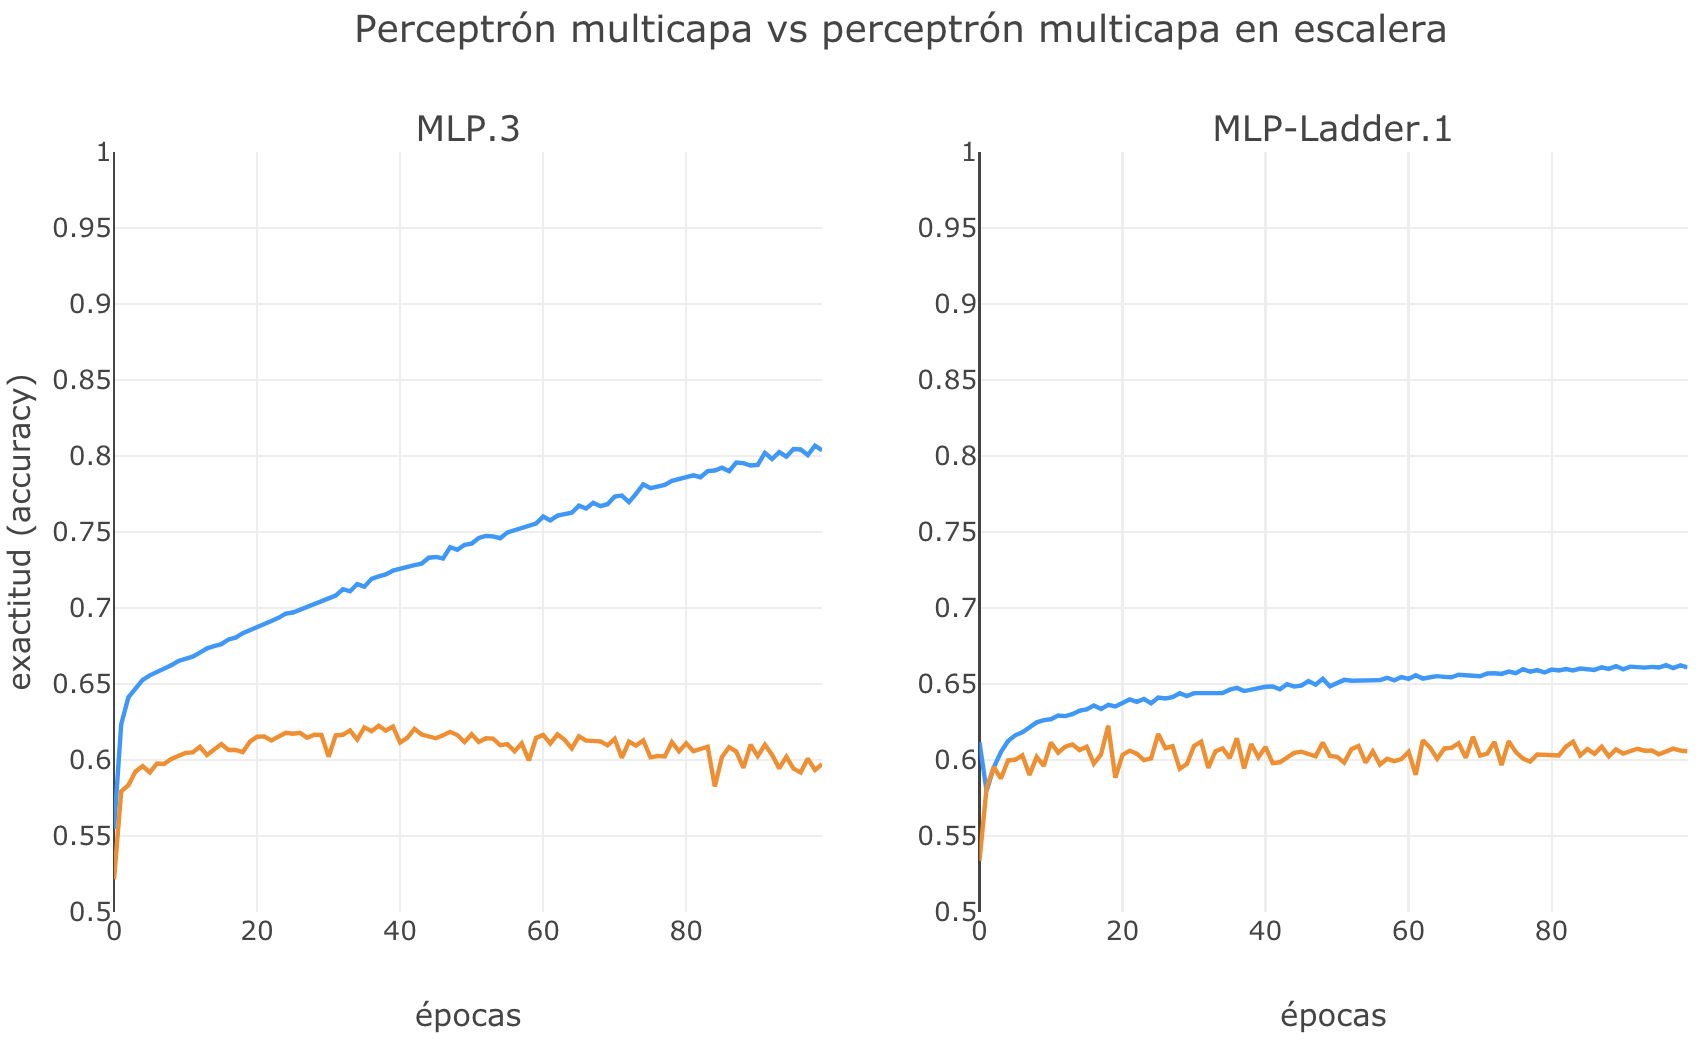
\includegraphics[width=.9\linewidth]{images/MLP_supervised_ladder.png}
\caption{Perceptrón multicapa supervisado vs semisupervisado (escalera). Comparación de evolución de
datos de entrenamiento y datos de validación}
\label{fig:MLP_supervised_ladder}
\end{center}
\end{figure}

En la Figura \ref{fig:MLP_supervised_ladder} se observan dos gráficos, las trazas azules describen el valor de
exactitud del modelo a lo largo de las épocas en los datos de entrenamiento y las trazas anaranjadas de manera
análoga en los datos de validación. El gráfico a izquierda corresponde al experimento MLP.3 que utiliza la 
estrategia de decaimiento exponencial para representar cada palabra y que consiguió el mejor desempeño en la 
Sección \ref{baseline:mlp}. 

Por otro lado, el gráfico a derecha es un experimento equivalente (i.e. con los mismos hiperparámetros y datos
de entrenamiento y validación) en su versión en escalera.

Se puede apreciar como el modelo en escalera permite una mejor generalización que el netamente supervisado al 
observar que la curva correspondiente a los datos de validación acompaña a la de entrenamiento (i.e. el `gap' entre entrenamiento y validación no es tan alto). Más aún, se observa como para el caso del experimento 
puramente supervisado, después de ciertas iteraciones el desempeño sobre validación comienza a caer. En el 
caso del experimento semi-supervisado, por el contrario, el desempeño entre entrenamiento y validación se 
mantiene bastante constante a lo largo del tiempo, lo que es un primer indicio de que el modelo 
semi-supervisado sirve para regularizar el modelo.

\subsubsection{Comparación de valores finales de desempeño sobre datos de entrenamiento vs. evaluación}

La figura \ref{fig:MLP_supervised_ladder_bar} muestra los valores de exactitud para los datos de entrenamiento
y evaluación de los modelos del perceptrón multicapa supervisado y su variante en escalera. 

Es un gráfico de barras con agrupación. El eje $y$ del gráfico muestra la exactitud ({\em accuracy}) del 
experimento, donde a mayor valor, mejor el resultado. Por otro lado, el eje $x$ representa el modelo 
utilizado, agrupando dos barras de acuerdo al conjunto de datos sobre el que se muestra el resultado. 

De esta manera, la barra azul muestra el resultado sobre el conjunto de entrenamiento y la barra verde sobre 
el conjunto de evaluación ({\em test}). Nuevamente se observa una mayor generalización por parte del modelo 
perceptrón multicapa en escalera ({\em MLP-Ladder.1}) ya que la diferencia en cuanto al desempeño en los datos
de evaluación y entrenamiento es notablemente menor, mientras que el desempeño en el conjunto de datos de 
evaluación para el método semi-supervisado es igual (sino mayor) al mostrado para el caso puramente 
supervisado. Junto con los resultados de la Figura \ref{fig:MLP_supervised_ladder}, podemos concluir que
el uso de datos no anotados en el modelo arroja resultados interesantes a la hora de regularizar dicho
modelo.

\begin{figure}[t]
\begin{center}
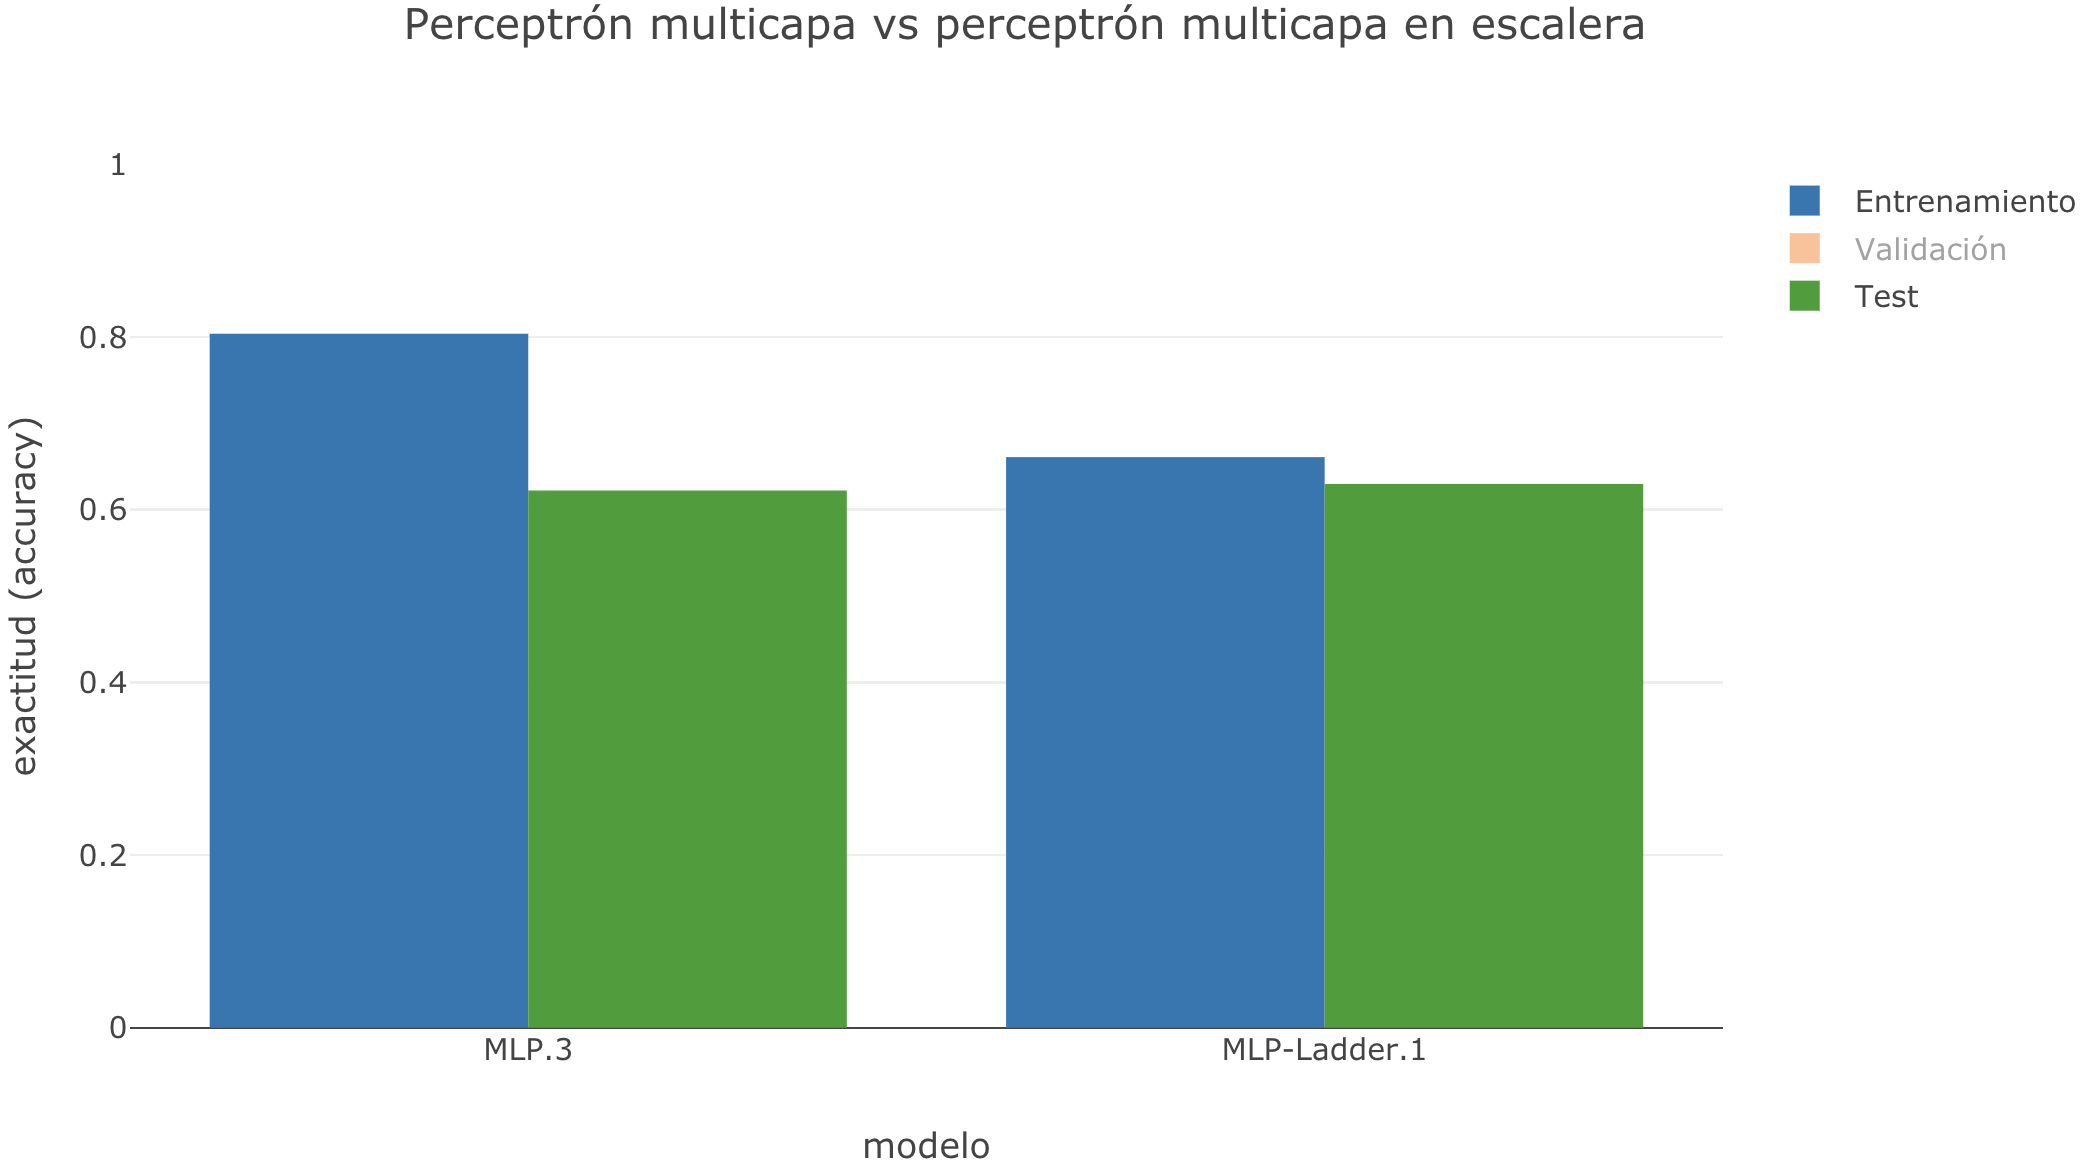
\includegraphics[width=.9\linewidth]{images/MLP_supervised_ladder_bar.png}
\caption{Perceptrón multicapa supervisado vs semisupervisado (escalera). Comparación de resultados finales
sobre datos de entrenamiento y datos de validación}
\label{fig:MLP_supervised_ladder_bar}
\end{center}
\end{figure}

\subsection{Impacto de selección de datos anotados y no anotados para el entrenamiento: Redes convolucionales 
en escalera en amplitud}

Este conjunto de experimentos busca medir el impacto de utilizar distintos tipos de datos de entrenamiento
para los modelos semi-supervisados de redes en escalera. En particular, nos interesa observar como se comporta
un modelo de red en escalera convolucional en amplitud a partir de la que se define en la Sección 
\ref{sec:cnn:wide}. 

Se observan distintas combinaciones de datos anotados y no anotados como entrenamiento para los modelos de la 
red convolucional en escalera. No obstante, se mantienen las mismas 20000 instancias de validación y 20000 de 
evaluación utilizadas en la versión supervisada para poder comparar con el baseline supervisado de la Sección 
\ref{baseline:cnn:wide}.

\begin{table}[b!]
    \centering
    \begin{tabular}{|l|l|l|}
        \hline
        \textbf{Experimento} & \textbf{Hiperparámetro} & \textbf{Valor} \\
        \hline
        \multirow{8}{*}{Hiper. generales} & Ventana simétrica W & 2 \\
                              & Número de filtros & 100 \\
                              & Factor de ruido por capa & 0.3 \\
                              & Costo de reducción de ruido & [100, 0.1, 0.01] \\
                              & Factor costo no supervisado & 0.3 \\
                              & Tasa de aprendizaje & 0.02 \\
                              & Tamaño de max pooling & 1 \\
                              & Tamaño de kernels & [2,3,4] \\
                              
        \hline
        \multirow{2}{*}{CNN-Wide-Ladder.1} & Datos anotados & 100k \\
                                           & Datos no anotados & mismos 100k \\
        \hline
        \multirow{2}{*}{CNN-Wide-Ladder.2} & Datos anotados & 100k \\
                                           & Datos no anotados & 100k disjuntos \\
        \hline
        \multirow{2}{*}{CNN-Wide-Ladder.3} & Datos anotados & 100k \\
                                           & Datos no anotados & 200k \\
        \hline
    \end{tabular}
    \caption{Hiperparámetros del conjunto de experimentos con redes convolucionales en amplitud en escalera.}
    \label{tab:exp:cnn_wide_ladder}
\end{table}

Notar que en estos casos, a diferencia del perceptrón multicapa de la sección anterior, un ejemplo de 
entrenamiento es un fragmento de oración como se detalla en la Sección \ref{sec:fragmento_sentencia}. 

El Cuadro \ref{tab:exp:cnn_wide_ladder} detalla los experimentos realizados con las redes convolucionales
en escalera en amplitud, basadas en lo detallado en la Sección \ref{sec:cnn:wide}.

Para el caso del modelo de redes convolucionales en amplitud en escalera se muestran tres experimentos, con 
los hiperparámetros generales que mejores resultados obtuvieron seleccionados de manera aleatoria. 

Lo que varían en estos experimentos son las instancias utilizadas para el entrenamiento del modelo, la razón 
de esto es medir el impacto que generan los datos no anotados dependiendo si coinciden o no con los anotados y
que sucede si variamos la proporción utilizada.

\subsubsection{Comparación de distintos tipos de datos de entrada: iguales, disjuntos y contenidos}

\begin{figure}[t]
\begin{center}
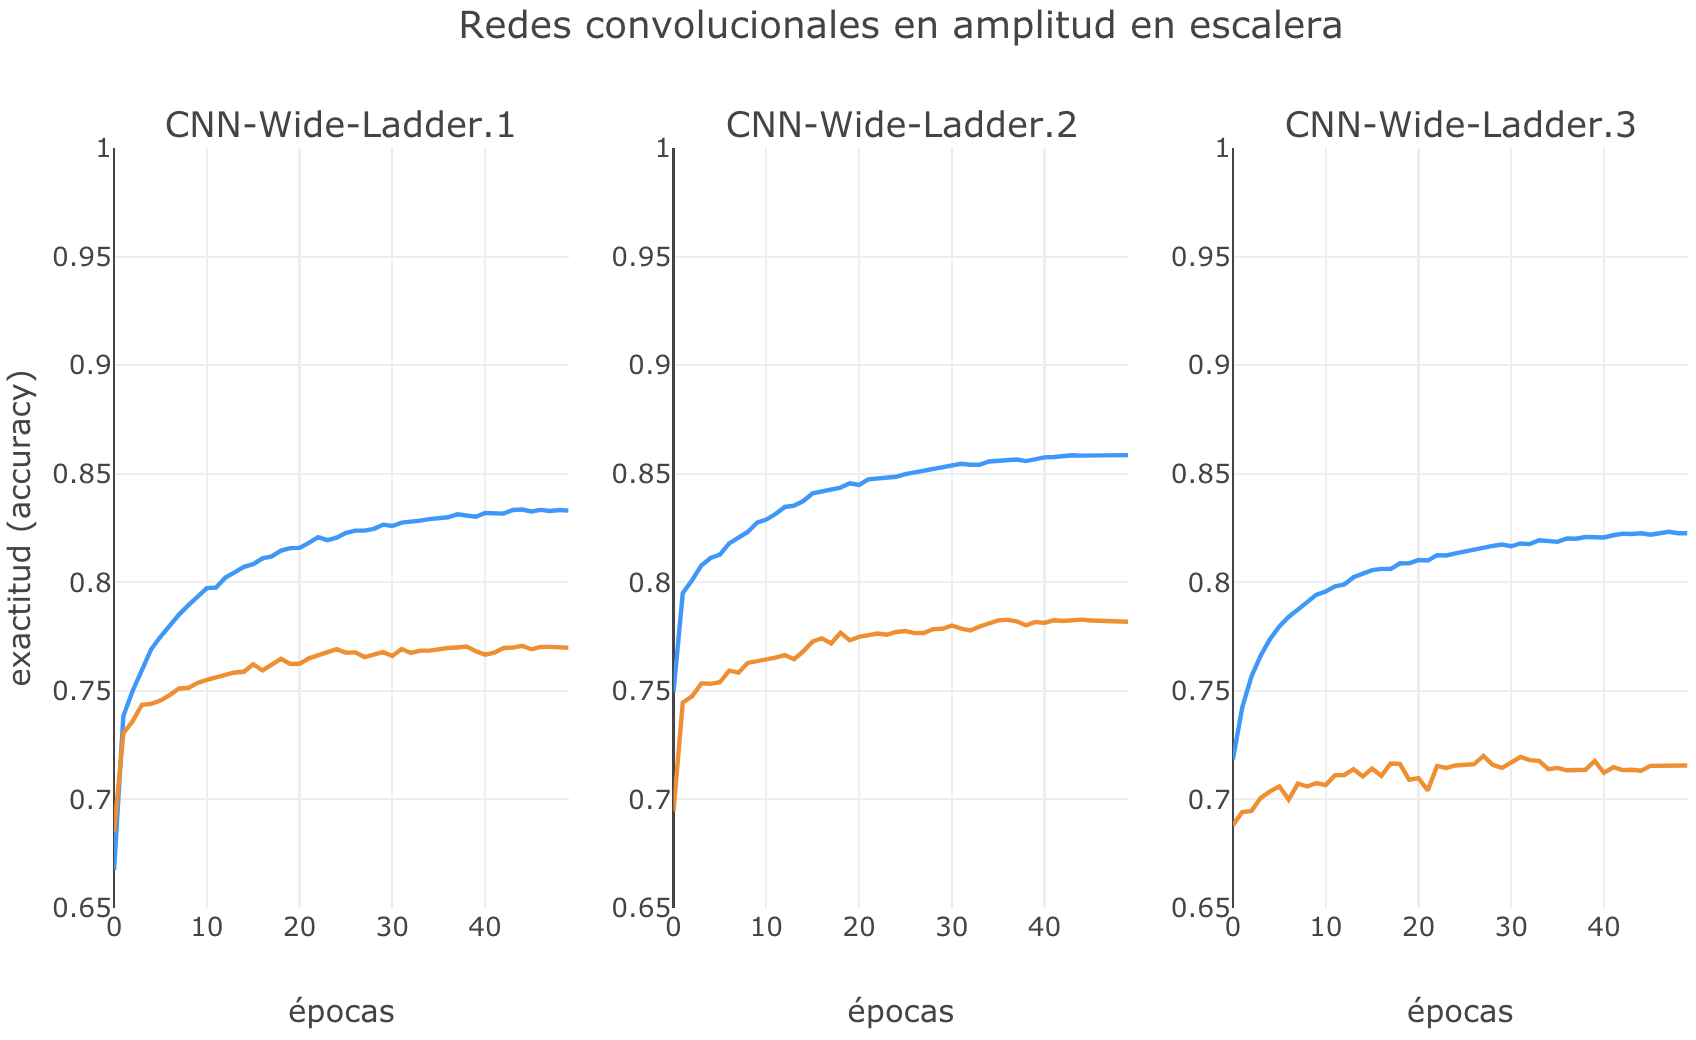
\includegraphics[width=.9\linewidth]{images/CNN_wide_ladder.png}
\caption{Redes convolucionales en amplitud en escalera. Comparación de resultados utilizando distintos
conjuntos de entrenamiento anotado y no anotado.}
\label{fig:CNN_wide_ladder}
\end{center}
\end{figure}

En la figura \ref{fig:CNN_wide_ladder} se observan tres gráficos correspondientes a los experimentos 
realizados sobre el modelo de redes convolucionales en amplitud en escalera. 

A izquierda se ubica el gráfico correspondiente a utilizar las mismas 100k instancias de entrenamiento como 
datos anotados y no anotados. 

El gráfico central es el resultante de haber utilizado 100k instancias anotadas y 100k instancias disjuntas no anotadas. 

Por último, el gráfico de la derecha utiliza las 100k instancias originales como datos anotados y no anotados 
y, a su vez, suma 100k nuevos no anotados. 

El experimento CNN-Wide-Ladder.2 nos muestra que agregar nuevos datos no anotados parece ser clave para 
mejorar el rendimiento del modelo. Sin embargo agregar demasiados datos no anotados puede afectar al modelo de
manera negativa como se observa en el experimento CNN-Wide-Ladder.3. Esto último puede deberse al hecho de que
la red no es lo suficientemente capaz de manejar la reconstrucción de tantos datos no anotados, quizás se 
requeriría una red de mayor tamaño para dicha tarea.

\subsubsection{Comparación de resultados supervisados y semi-supervisados en la evolución de entrenamiento vs.
validación por épocas}

La Figura \ref{fig:CNN_wide_supervised_ladder} hace una comparación del mejor modelo obtenido en
la Sección \ref{baseline:cnn:wide} y el modelo obtenido con CNN-Wide-Ladder.2. 

\begin{figure}[t]
\begin{center}
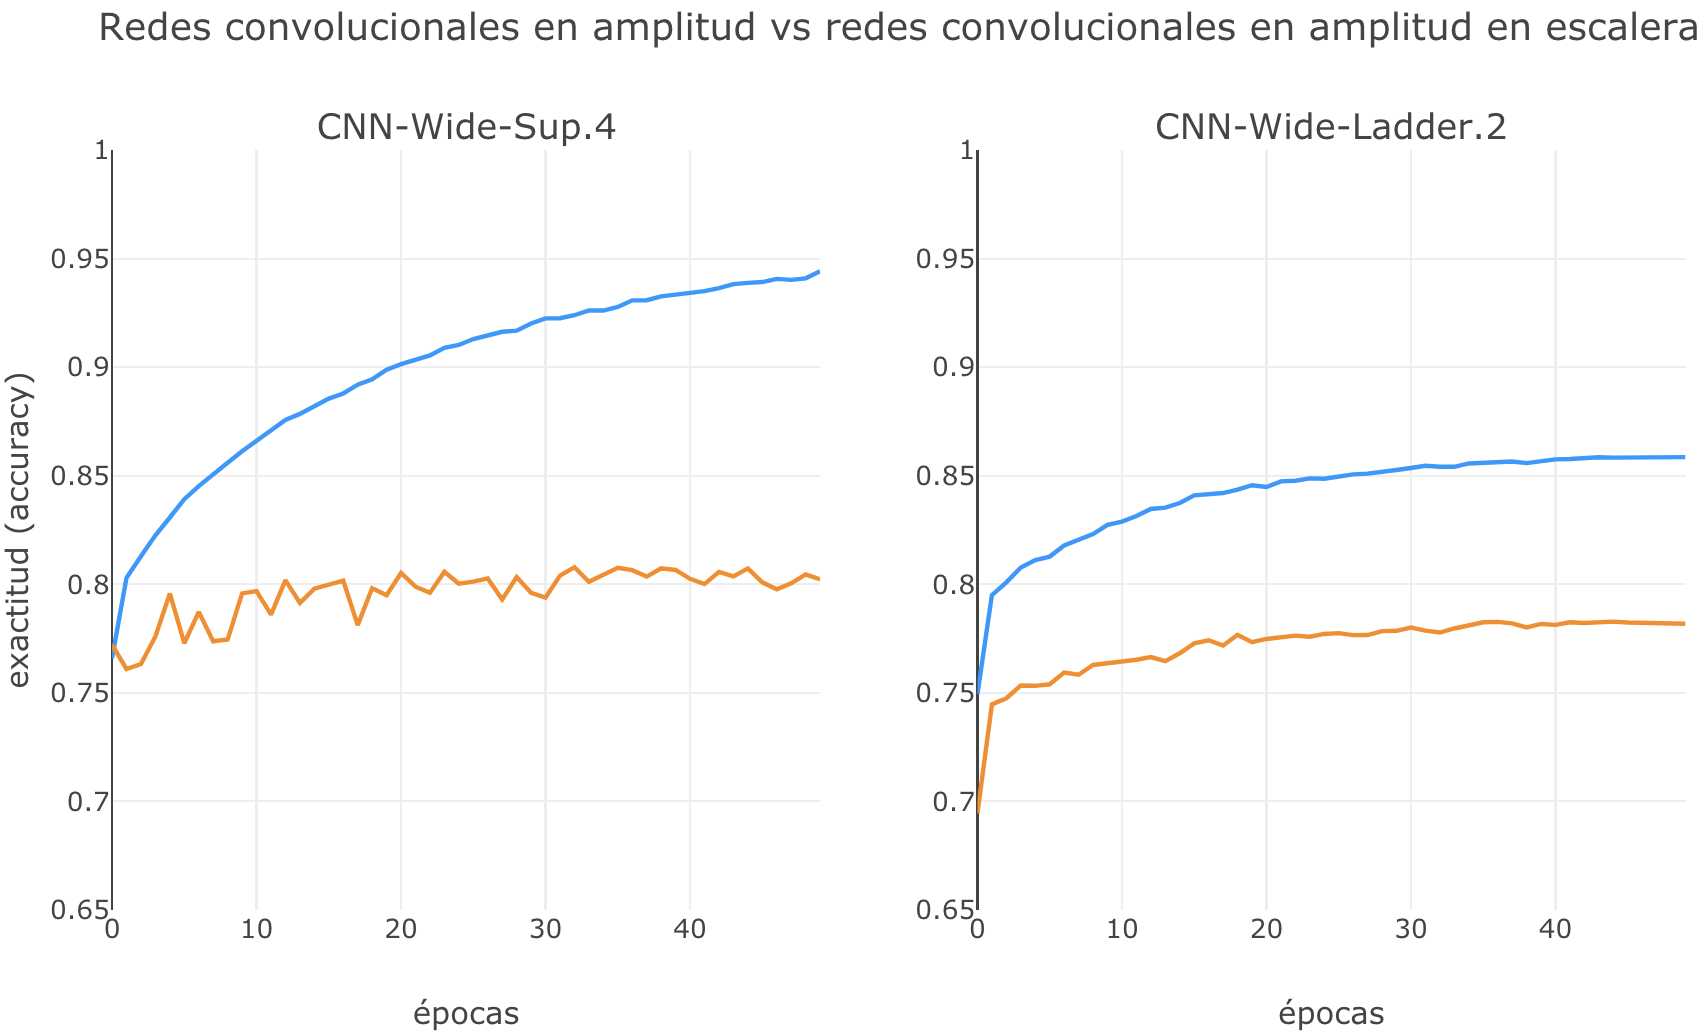
\includegraphics[width=.9\linewidth]{images/CNN_wide_supervised_ladder.png}
\caption{Modelo de redes convolucionales en amplitud supervisado vs semi-supervisado (escalera). Comparación
de evolución en épocas del desempeño en corpus de entrenamiento y corpus de validación.}
\label{fig:CNN_wide_supervised_ladder}
\end{center}
\end{figure}

Como se puede observar, la implementación del modelo de redes convolucionales en amplitud en escalera, la 
curva anaranjada (validación) acompaña a una distancia más cercana a la curva azul (entrenamiento) que en el 
caso del modelo supervisado. 

Más aún, si bien en este caso el desempeño del modelo semisupervisado sobre el conjunto de datos de validación
es ligeramente menor que para el modelo puramente supervisado (medido mediante la exactitud), se muestra menor
ruido en el desempeño.

De manera análoga al modelo perceptrón multicapa en escalera, se comprueba que la tarea no supervisada 
colabora en la generalización del modelo.

\subsubsection{Comparación de precisión y exhaustividad por clase supervisados y semi-supervisados con 
resultados sobre datos de evaluación}

Finalmente, para una comparación más detallada, con métricas de precisión y exhaustividad ({\em precisión \& 
recall}), la Figura \ref{fig:CNN_wide_supervised_ladder_precision_recall} presenta una comparación clase por 
clase entre los dos modelos para el conjunto de datos de evaluación. En el gráfico, cada cuarto representa la 
clase a comparar (PER, LOC, ORG, y MISC, la clase O no se compara). Es un gráfico de barras agrupadas de 
acuerdo al modelo (redes convolucionales en amplitud supervisadas y no supervisadas).

La barra de color rojo representa el valor de exhaustividad que obtuvo cada modelo para cada clase en 
particular sobre el conjunto de datos de evaluación. La barra de color color ocre representa los valores de 
precisión obtenidos. No se observan grandes diferencias entre los modelos, con el modelo supervisado superando
en algunos casos al semi-supervisado y viceversa. Posteriormente se utilizarán estos resultados para su 
comparación con el modelo de redes convolucionales en profundidad.

\begin{figure}[h]
\begin{center}
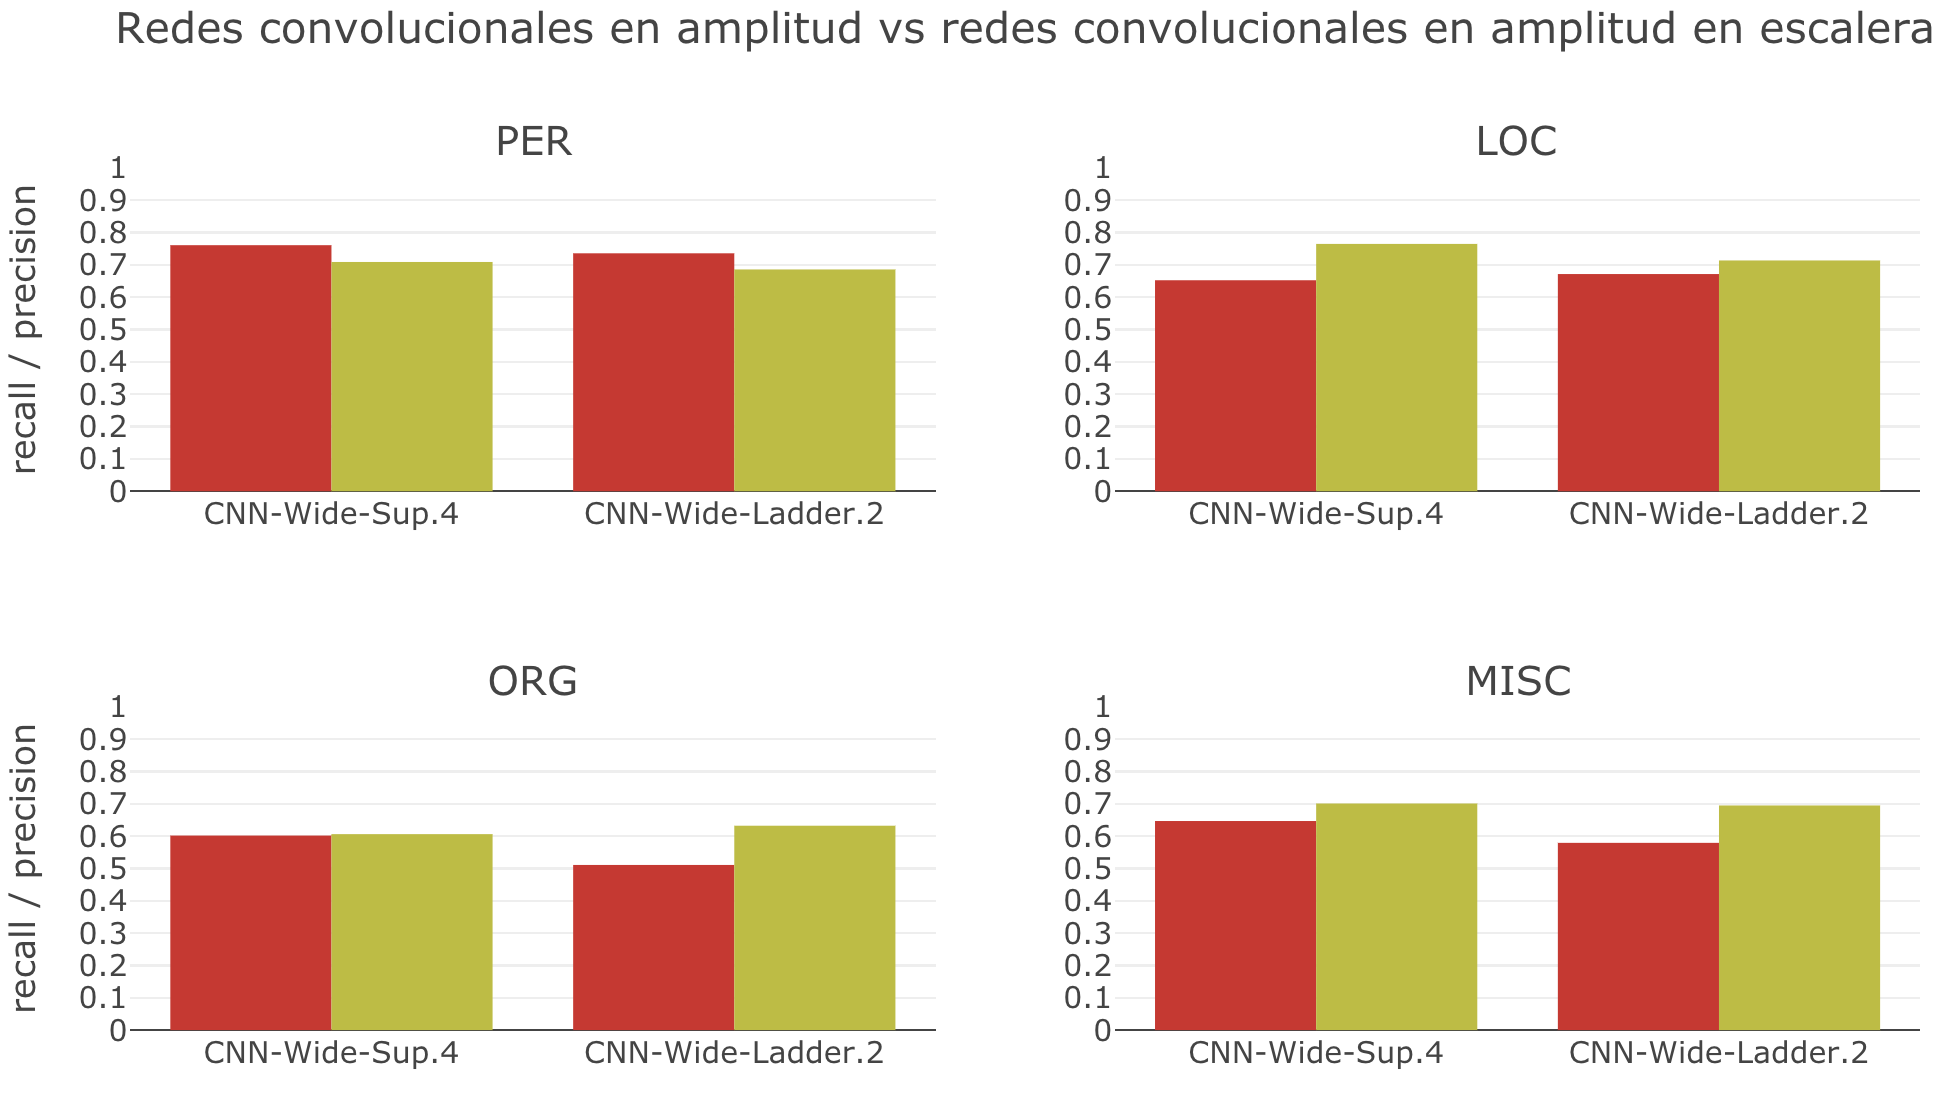
\includegraphics[width=.9\linewidth]{images/CNN_wide_supervised_ladder_precision_recall.png}
\caption{Modelo de redes convolucionales en amplitud supervisado vs semi-supervisado (escalera). Comparación
de desempeño mediante precisión y exhaustividad por clase sobre conjunto de datos de evaluación.}
\label{fig:CNN_wide_supervised_ladder_precision_recall}
\end{center}
\end{figure}

\subsection{Impacto de datos anotados para entrenamiento: Redes convolucionales
en escalera en profundidad}

En esta serie de experimentos buscamos medir el impacto del desempeño del modelo modificando la cantidad
inicial de datos anotados sobre los cuales entrenar la parte supervisada del modelo. 

Como caso de estudio, se utilizaron las redes convolucionales en escalera en profundidad definidas en la 
Sección \ref{sec:cnn:deep}, ya que en estas el desempeño de la parte supervisada del modelo era esencial 
puesto que no se pueden, por la naturaleza de los datos secuenciales, subsamplear la clase mayoritarias ``O''.
Por lo que queremos ver efectivamente que tan importante es el uso de datos anotados para el desempeño general
del modelo semi-supervisado.

\begin{table}[b!]
    \centering
    \begin{tabular}{|l|l|l|}
        \hline
        \textbf{Experimento} & \textbf{Hiperparámetro} & \textbf{Valor} \\
        \hline
        \multirow{10}{*}{Hiper. generales} & Número de filtros & 100 \\
                              & Capas convolucionales & 10 \\
                              & Factor de ruido por capa & 0.3 \\
                              & Costo ruido capa de entrada & 100 \\
                              & Costo ruido capa convolucional & 0.1 \\
                              & Costo ruido capa de salida & 0.01 \\
                              & Factor costo no supervisado & 0.1 \\
                              & Tasa de aprendizaje & 0.02 \\
                              & Tamaño de kernels & 2 \\
                              & Datos entrenamiento no anotados & 100k \\
                              
        \hline
        \multirow{1}{*}{CNN-Depth-Ladder-a} & Datos entrenamiento anotados & 25k \\
        \hline
        \multirow{1}{*}{CNN-Depth-Ladder-b} & Datos entrenamiento anotados & 50k \\
        \hline
        \multirow{1}{*}{CNN-Depth-Ladder-c} & Datos entrenamiento anotados & 75k \\
        \hline
        \multirow{1}{*}{CNN-Depth-Ladder-d} & Datos entrenamiento anotados & 100k \\
        \hline
    \end{tabular}
    \caption{Hiperparámetros del conjunto de experimentos con redes convolucionales en profundidad en escalera.}
    \label{tab:exp:cnn_depth_ladder}
\end{table}

En los experimentos se varía la proporción de datos anotados en la etapa de entrenamiento con la 
promesa de que el modelo semi-supervisado puede suplir la falta de datos anotados gracias al uso de datos no 
anotados. En estos experimentos, al utilizarse un modelo de etiquetado de secuencias, se evalúan datos
del tipo ``Oración - Etiquetas'' como se definen en la Sección \ref{sec:sequence_labeling}. Notar que este experimento también se realizó en otras arquitecturas en escalera con resultados similares pero con fines de no ser reiterativos se decidió mostrar los resultados para esta arquitectura en particular.

En el Cuadro \ref{tab:exp:cnn_depth_ladder}, se detallan los cuatro experimentos realizados, con los 
hiperparámetros generales que mejores resultados obtuvieron seleccionados de manera aleatoria. Lo que varía 
son las instancias anotadas utilizadas para el entrenamiento del modelo. No obstante, se decidió mostrar únicamente la comparación entre los modelos CNN-Depth-Ladder-a y CNN-Depth-Ladder-d que mostraban los resultados mas relevantes en cuanto a la validación de la hipótesis propuesta.

\subsubsection{Comparación de resultados semi-supervisados al variar la proporción de datos anotados para el entrenamiento.}

En la Figura \ref{fig:CNN_depth_ladder_precision_recall} se observan los valores de \textit{recall} (en color rojo) y de \textit{precision} (en color verde claro) para cada una de las clases que representan una entidad nombrada sobre el conjunto de evaluación. Se compara el modelo de redes convolucionales en profundidad en escalera utilizando 25000 instancias etiquetadas (CNN-Depth-Ladder-a) contra utilizar 100000 instancias etiquetadas (CNN-Depth-Ladder-d) para el entrenamiento del modelo. En general, se obtiene entre 1 y 2 puntos de mejora al utilizar la totalidad de ejemplos etiquetados salvo para los casos de \textit{precision} en la clase PER y de \textit{recall} en la clase MISC donde incluso tomar una proporción menor (25\%) del total de instancias de entrenamiento generó mejores resultados. Vemos entonces la ventaja de trabajar con este modelo semi-supervisado donde tomar una proporción significativamente menor de datos para el entrenamiento no se corresponde con una gran pérdida de desempeño.

\begin{figure}[H]
\begin{center}
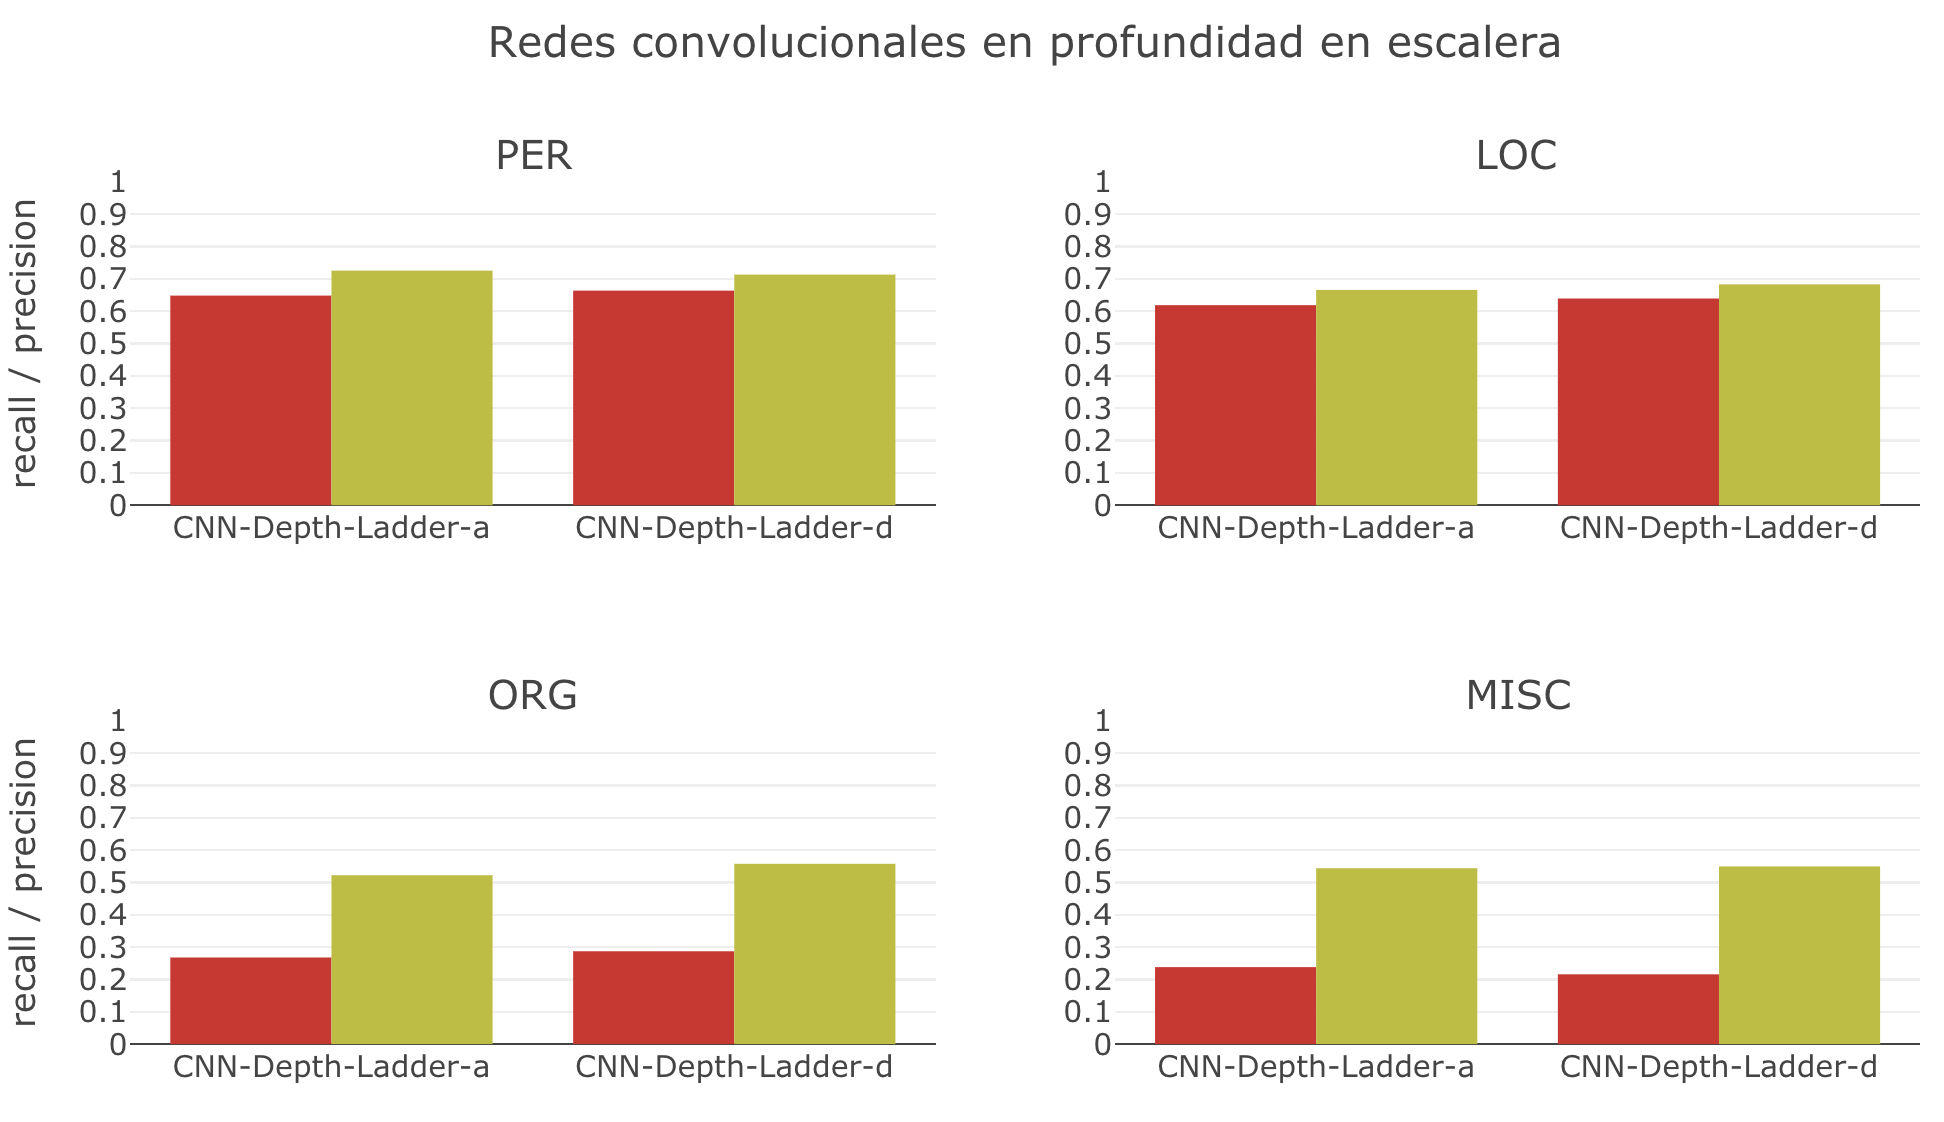
\includegraphics[width=.9\linewidth]{images/CNN_depth_ladder_precision_recall.png}
\caption{Redes convolucionales en profundidad en escalera.}
\label{fig:CNN_depth_ladder_precision_recall}
\end{center}
\end{figure}

\subsubsection{Comparación de mejores resultados de los modelos de redes convolucionales en amplitud y profundidad en escalera.}

En la Figura \ref{fig:CNN_wide_depth_ladder_precision_recall} se comparan los mejores resultados de los modelos de redes convolucionales en amplitud y en profundidad ambos en su variante en escalera. El color rojo se utiliza para los valores de \textit{recall} y el verde claro para los valores de \textit{precision} alcanzados por cada uno de los modelos en sus correspondientes conjuntos de evaluación. El modelo de redes convolucionales posee un desempeño superior visible en todas las clases y de manera más notable en las categorías ORG y MISC, sólo en el caso de \textit{precision} para la categoria PER el modelo de redes convolucionales en profundidad es ligeramente superior.

\begin{figure}[H]
\begin{center}
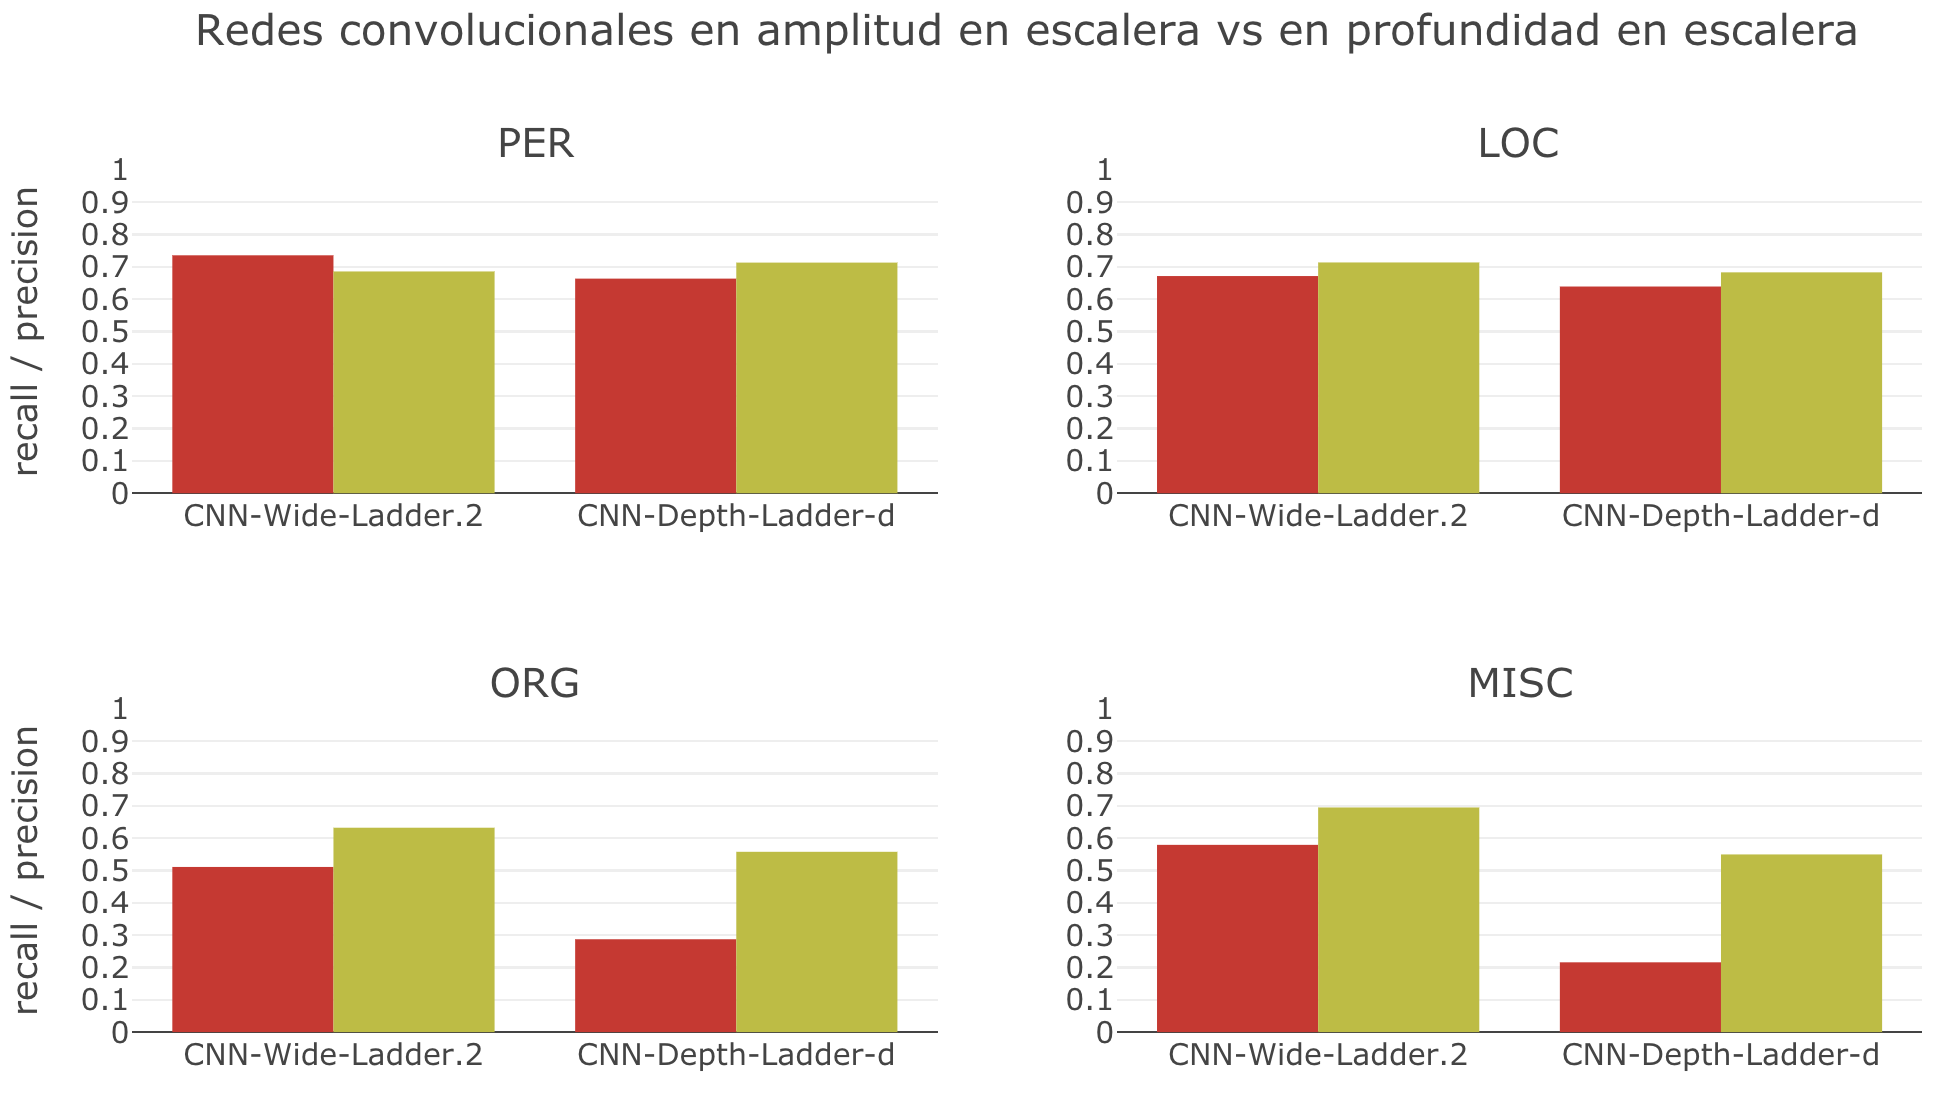
\includegraphics[width=.9\linewidth]{images/CNN_wide_depth_ladder_precision_recall.png}
\caption{Redes convolucionales en amplitud en escalera vs en profundidad en escalera.}
\label{fig:CNN_wide_depth_ladder_precision_recall}
\end{center}
\end{figure}

\subsection{Impacto del costo no supervisado en el aprendizaje del modelo: Redes convolucionales en escalera en profundidad}

Una hipótesis que surgió a lo largo de este trabajo fue si brindar demasiada importancia a la tarea no supervisada perjudica el entrenamiento del modelo ya que el mismo se concentraría en la reconstrucción de la entrada en lugar de la tarea prioritaria de predicción. Para ello, se agregó un factor $\mu$ detallado en \ref{sec:ladder_net} que nos permitiera ajustar el peso del costo no supervisado. 

\begin{table}[H]%[b!]
    \centering
    \begin{tabular}{|l|l|l|}
        \hline
        \textbf{Experimento} & \textbf{Hiperparámetro} & \textbf{Valor} \\
        \hline
        \multirow{10}{*}{Hiper. generales} & Número de filtros & 100 \\
                              & Capas convolucionales & 10 \\
                              & Factor de ruido por capa & 0.3 \\
                              & Costo ruido capa de entrada & 100 \\
                              & Costo ruido capa convolucional & 0.1 \\
                              & Costo ruido capa de salida & 0.01 \\
                              & Factor costo no supervisado & 0.1 \\
                              & Tasa de aprendizaje & 0.02 \\
                              & Tamaño de kernels & 2 \\
                              & Datos entrenamiento no anotados & 100k \\
                              
        \hline
        \multirow{1}{*}{u\_cost 0} & Valor de \mu & 0 \\
        \hline
        \multirow{1}{*}{u\_cost 0.1} & Valor de \mu & 0.1 \\
        \hline
        \multirow{1}{*}{u\_cost 0.3} & Valor de \mu & 0.3 \\
        \hline
        \multirow{1}{*}{u\_cost 0.5} & Valor de \mu & 0.5 \\
        \hline
    \end{tabular}
    \caption{Hiperparámetros del conjunto de experimentos con redes convolucionales en profundidad en escalera.}
    \label{tab:exp:cnn_depth_ladder_loss}
\end{table}

\subsubsection{Comparación de las curvas de loss durante el entrenamiento del modelo.}

En la Figura \ref{fig:CNN_depth_ladder_loss} se observan los resultados de cuatro experimentos realizados sobre el modelo de redes convolucionales en profundidad en escalera. El valor u\_cost es un factor multiplicativo aplicado a la función de costo no supervisada del modelo (denotado como $\mu$ en la sección \ref{sec:ladder_net}). Por lo cual, a mayor u\_cost mayor es la ponderación que se le da a la función de costo no supervisada que el modelo debe minimizar conjuntamente con la supervisada. El color azul representa el valor de pérdida (\textit{loss}) supervisado del modelo a lo largo de las épocas sobre el conjunto de entrenamiento mientras que el anaranjado sobre el conjunto de validación. Es importante tener en consideración no darle demasiado peso a la función de costo no supervisada, ya que provoca que el modelo se centre demasiado en la tarea de reconstrucción dejando de lado la tarea supervisada de clasificación. Se observa como con un u\_cost de 0.5 ya el modelo diverge.

\begin{figure}[t]
\begin{center}
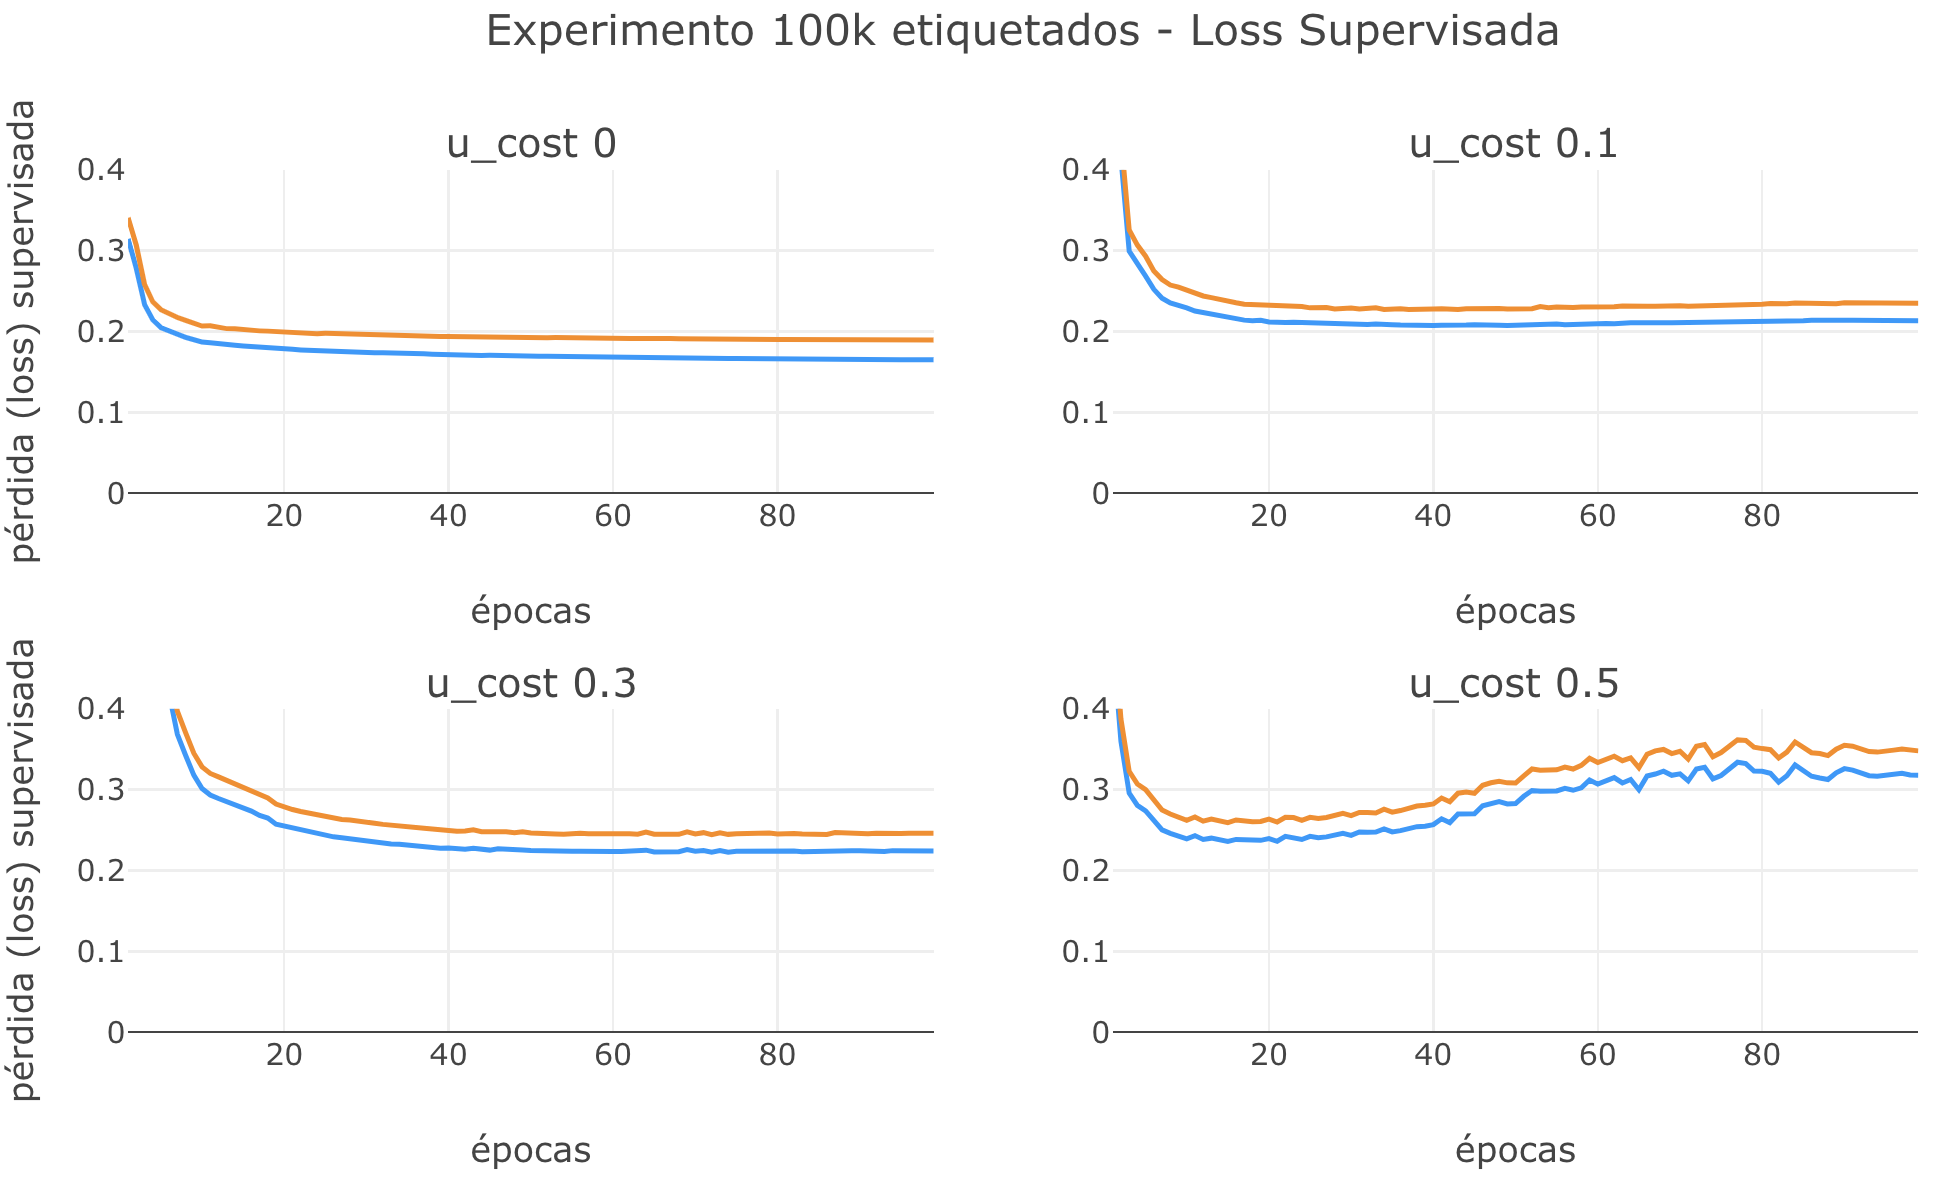
\includegraphics[width=.9\linewidth]{images/CNN_depth_ladder_loss.png}
\caption{Redes convolucionales en escalera experimento CNN-Depth-Ladder-d con variando el factor de la función de costo no supervisado.}
\label{fig:CNN_depth_ladder_loss}
\end{center}
\end{figure}

\subsection{Resultados finales}
% \vspace{5.0mm}

En los Cuadros \ref{table:best_train_CNN_results_table} y \ref{table:best_test_CNN_results_table} se comparan los mejores resultados utilizando la métrica F1-score de los modelos convolucionales. Se observa como los modelos supervisados superan a sus variantes en escalera y que la arquitectura del modelo de redes convolucionales en amplitud performa mejor al modelo de redes convolucionales en profundidad.

\begin{table}[H]
\begin{tabular}{|l|l|l|l|l|l|}
\hline
                    & PER    & LOC    & ORG    & MISC   & O      \\ \hline
CNN wide supervised & \textbf{0.9849} & \textbf{0.9751} & \textbf{0.9775} & \textbf{0.9753} & \textbf{0.9909} \\ \hline
CNN wide ladder     & 0.8152   & 0.8137 & 0.7453  & 0.7194 & 0.9269  \\ \hline
CNN depth supervised & 0.7923 & 0.7847 & 0.6953 & 0.6173 & 0.9837 \\ \hline
CNN depth ladder    & 0.6994 & 0.6628 & 0.4025 & 0.3261 & 0.9732 \\ \hline
\end{tabular}
\caption{F1-score de los mejores modelos por clase sobre los conjuntos de \textbf{entrenamiento} de cada uno de ellos.}
\label{table:best_train_CNN_results_table}
\end{table}


\begin{table}[H]
\begin{tabular}{|l|l|l|l|l|l|}
\hline
                    & PER    & LOC    & ORG    & MISC   & O      \\ \hline
CNN wide supervised & \textbf{0.7341} & 0.7042 & \textbf{0.6039} & \textbf{0.6726} & 0.9325 \\ \hline
CNN wide ladder     & 0.71   & 0.6921 & 0.565  & 0.6317 & 0.906  \\ \hline
CNN depth supervised & 0.7326 & \textbf{0.7089} & 0.5828 & 0.4897 & \textbf{0.9789} \\ \hline
CNN depth ladder    & 0.6876 & 0.6605 & 0.3791 & 0.3099 & 0.9696 \\ \hline
\end{tabular}
\caption{F1-score de los mejores modelos por clase sobre los conjuntos de \textbf{evaluación} de cada uno de ellos.}
\label{table:best_test_CNN_results_table}
\end{table}

Las Figuras \ref{fig:CNN_wide_supervised_ladder_F1-score} y \ref{fig:CNN_depth_supervised_ladder_F1-score} muestran los valores de F1-score para los datos de entrenamiento y evaluación comparando los modelos supervisados y en escalera de los modelos que utilizan las capas convolucionales en amplitud y en profundidad. En ambos casos nuevamente se observa la capacidad de generalización que aporta la tarea no supervisada de los modelos en escalera donde los valores obtenidos sobre el conjunto de evaluación son cercanos al conjunto de entrenamiento.

\begin{figure}[H]
\begin{center}
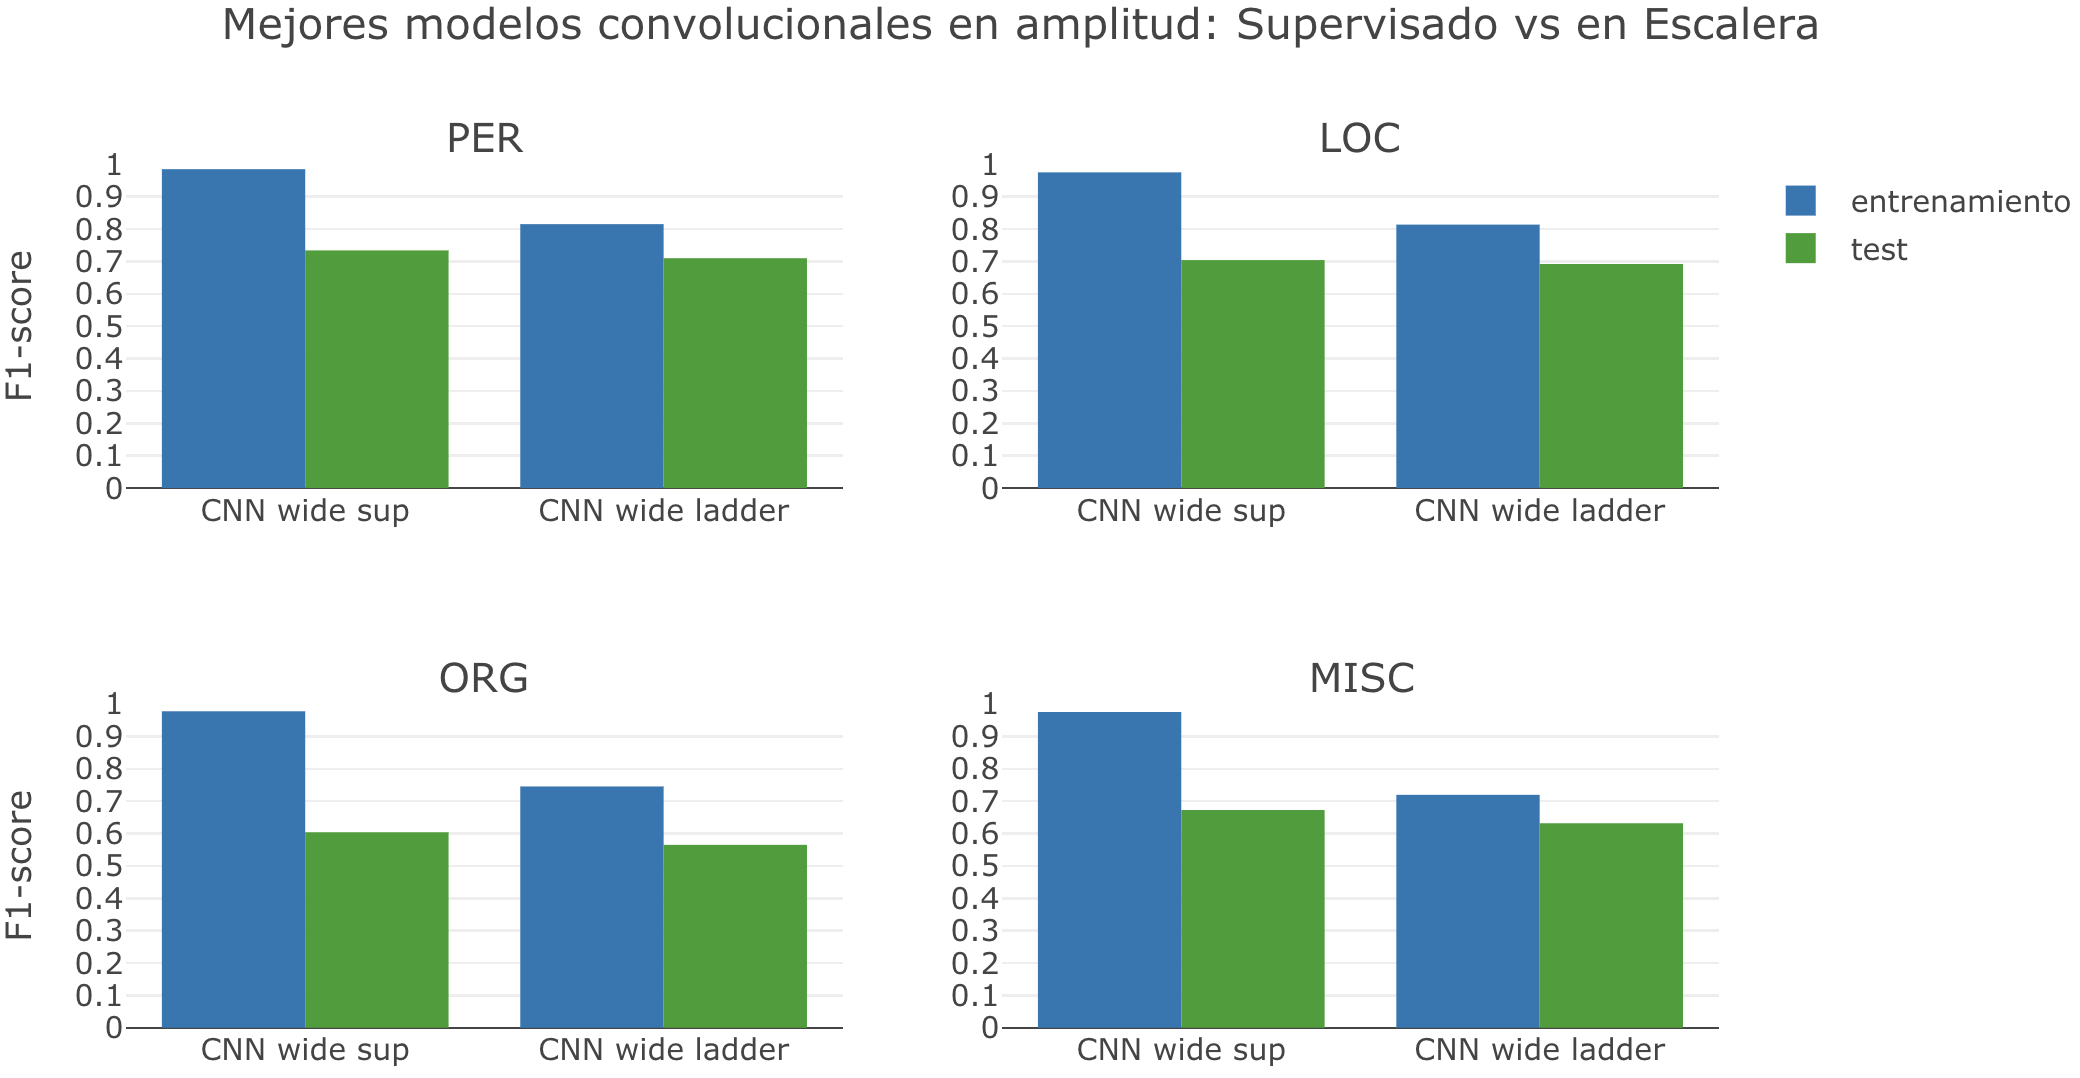
\includegraphics[width=.9\linewidth]{images/CNN_wide_supervised_ladder_F1-score.png}
\caption{}
\label{fig:CNN_wide_supervised_ladder_F1-score}
\end{center}
\end{figure}


\begin{figure}[H]
\begin{center}
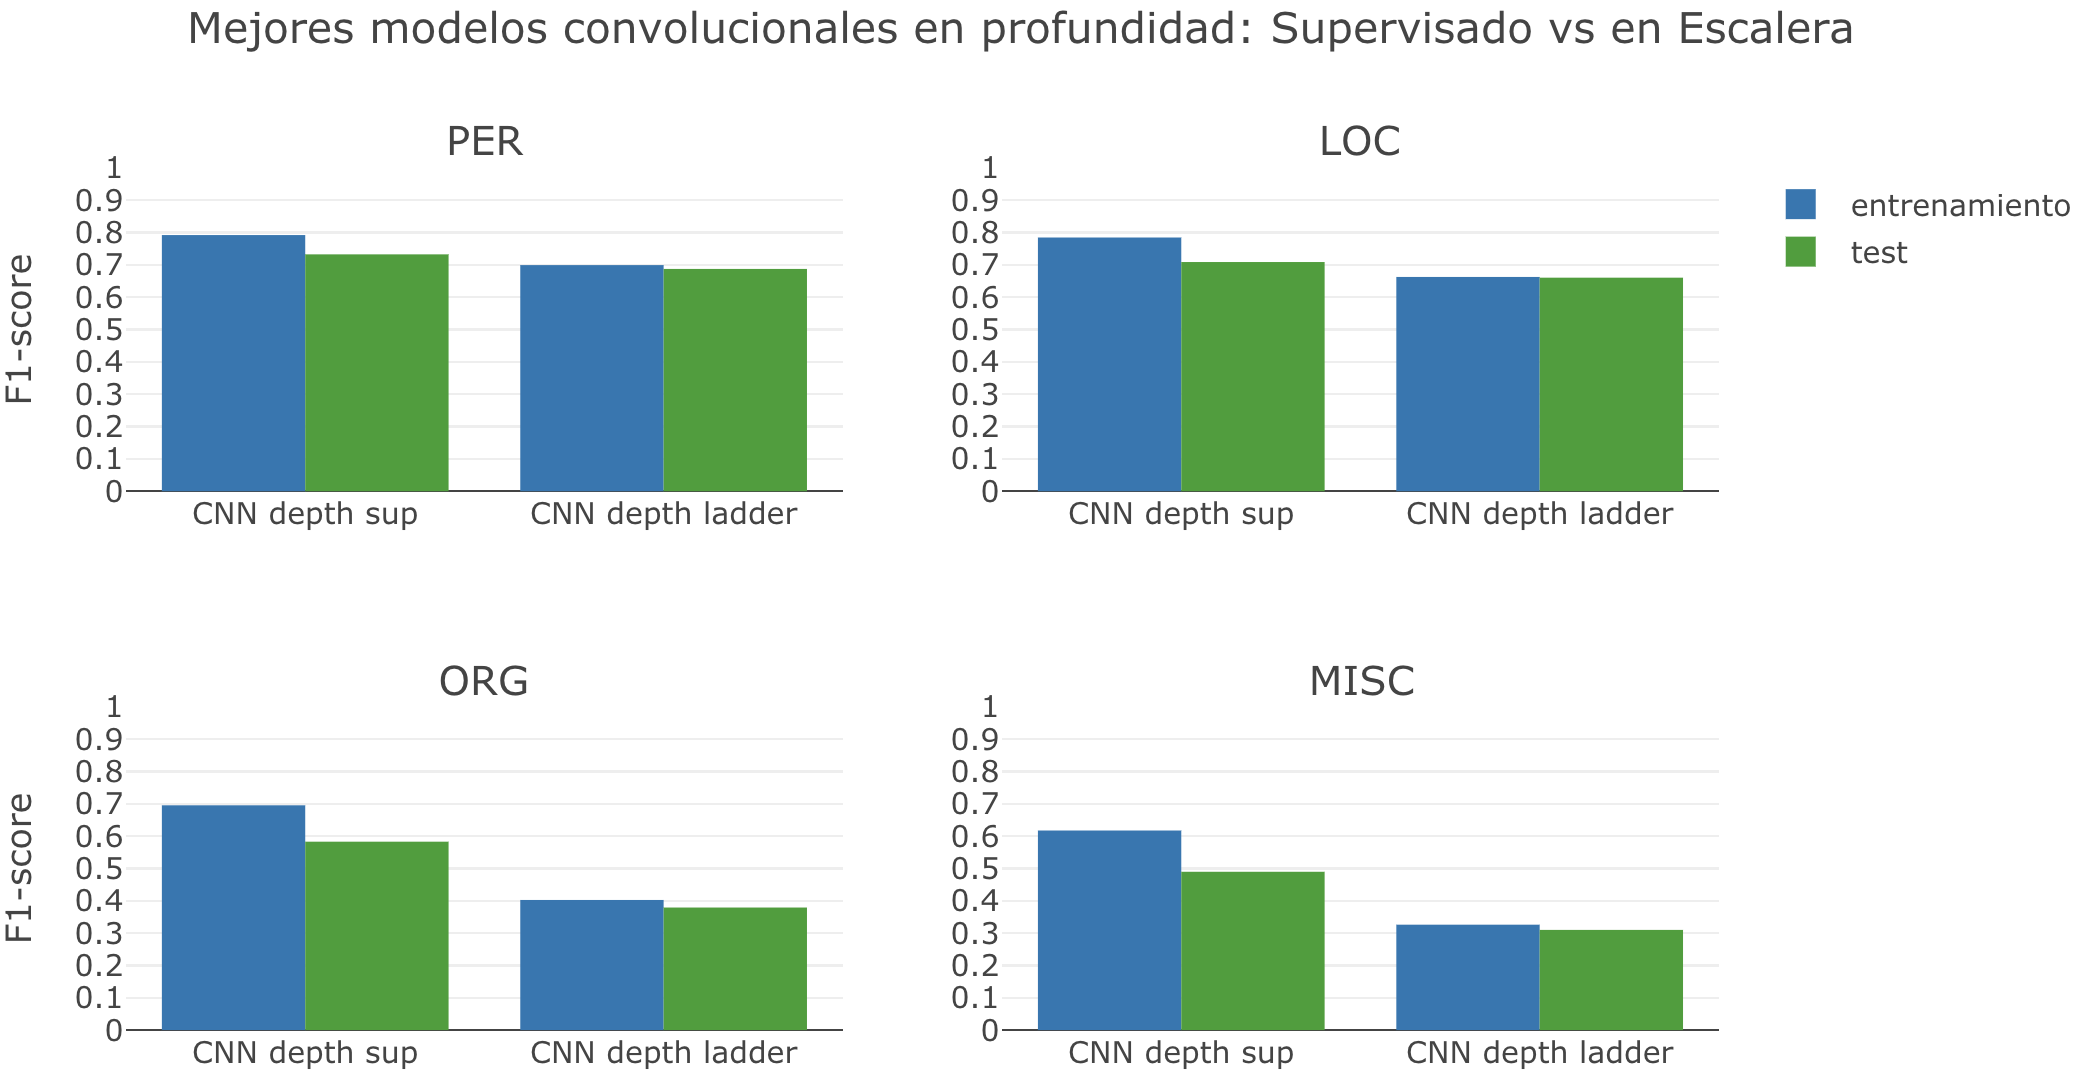
\includegraphics[width=.9\linewidth]{images/CNN_depth_supervised_ladder_F1-score.png}
\caption{}
\label{fig:CNN_depth_supervised_ladder_F1-score}
\end{center}
\end{figure}